%
%
% UCSD Doctoral Dissertation Template
% -----------------------------------
% http://ucsd-thesis.googlecode.com
%
%
% ----------------------------------------------------------------------
% WARNING: 
%
%   This template has not endorced by OGS or any other official entity.
%   The official formatting guide can be obtained from OGS.
%   It can be found on the web here:
%   http://ogs.ucsd.edu/AcademicAffairs/Documents/Dissertations_Theses_Formatting_Manual.pdf
%
%   No guaranty is made that this LaTeX class conforms to the official UCSD guidelines.
%   Make sure that you check the final document against the Formatting Manual.
%  
%   That being said, this class has been routinely used for successful 
%   publication of doctoral theses.  
%
%   The ucsd.cls class files are only valid for doctoral dissertations.
%
%
% ----------------------------------------------------------------------
% GETTING STARTED:
%
%   Lots of information can be found on the project wiki:
%   http://code.google.com/p/ucsd-thesis/wiki/GettingStarted
%
%
%   To make a pdf from this template use the command:
%     pdflatex template
%
%
%   To get started please read the comments in this template file 
%   and make changes as appropriate.
%
%   If you successfully submit a thesis with this package please let us
%   know.
%
%
% ----------------------------------------------------------------------
% KNOWN ISSUES:
%
%   Currently only the 12pt size conforms to the UCSD requirements.
%   The 10pt and 11pt options make the footnote fonts too small.
%
%
% ----------------------------------------------------------------------
% HELP/CONTACT:
%
%   If you need help try the ucsd-thesis google group:
%   http://groups.google.com/group/ucsd-thesis
%
%
% ----------------------------------------------------------------------
% BUGS:
%
%   Please report all bugs at:
%   http://code.google.com/p/ucsd-thesis/issues/list
%
%
% ----------------------------------------------------------------------
% More control of the formatting of your thesis can be achieved through
% modifications of the included LaTeX class files:
%
%   * ucsd.cls    -- Class file
%   * uct10.clo   -- Configuration files for font sizes 10pt, 11pt, 12pt
%     uct11.clo                            
%     uct12.clo
%
% ----------------------------------------------------------------------



% Setup the documentclass 
% default options: 12pt, oneside, final
%
% fonts: 10pt, 11pt, 12pt -- are valid for UCSD dissertations.
% sides: oneside, twoside -- note that two-sided theses are not accepted 
%                            by OGS.
% mode: draft, final      -- draft mode switches to single spacing, 
%                            removes hyperlinks, and places a black box
%                            at every overfull hbox (check these before
%                            submission).
% chapterheads            -- Include this if you want your chapters to read:
%                              Chapter 1
%                              Title of Chapter
%
%                            instead of
%                              1 Title of Chapter
\documentclass[12pt,chapterheads]{ucsd}



% Include all packages you need here.  
% Some standard options are suggested below.
%
% See the project wiki for information on how to use 
% these packages. Other useful packages are also listed there.
%
%   http://code.google.com/p/ucsd-thesis/wiki/GettingStarted



%% AMS PACKAGES - Chances are you will want some or all 
%    of these if writing a dissertation that includes equations.
%  \usepackage{amsmath, amscd, amssymb, amsthm}

%% GRAPHICX - This is the standard package for 
%    including graphics for latex/pdflatex.
\usepackage{scrextend}
\usepackage{pslatex}
\usepackage{graphicx}
\usepackage{tabularx}
\usepackage{pbox}






%% KDD
\usepackage{wrapfig}
\usepackage{balance}  % for \balance command ON LAST PAGE  (only there!)
%\usepackage{algorithmic}
%\usepackage{algorithm}
\usepackage[lined]{algorithm2e}
\usepackage{multirow}
\usepackage{subfigure}
\usepackage{graphicx}
\usepackage{caption}
\usepackage{amsmath}
\usepackage{amssymb}
\usepackage{amsfonts}
\usepackage{xspace}
\usepackage{url}
\usepackage{KDD/tweaklist}
\usepackage[show]{KDD/chato-notes}
\usepackage{color}
\usepackage{hyperref}

\newcommand{\spara}[1]{\smallskip\noindent{\bf #1}}
\newcommand{\mpara}[1]{\medskip\noindent{\bf #1}}  
\newcommand{\para}[1]{\noindent{\bf #1}}
\newcommand{\IGNORE}[1]{}

\newcommand{\yahoo}{{\sf Yahoo!}}
    
%\renewcommand{\enumhook}{\setlength{\topsep}{0.2pt}
%\setlength{\itemsep}{0pt}}

\newcommand{\alg}[1]{\bigbreak\noindent{\bf #1}}
\newcommand{\algskip}{\itemsep=-8pt\baselineskip=0pt}
\newcommand{\commentedtext}[1]{}
\newcommand{\myalgostyle}[1]  {{#1}\xspace}
%% my algorithms
\newcommand{\optselect}{\myalgostyle{OptSelect}}
%\newcommand{\optselect}{OptSelect\xspace}
\newcommand{\M}{$\mathbf{M}$}
\newtheorem{example}{Example}
\newtheorem{definition}{Definition}
\newtheorem{theorem}{Theorem}
\newtheorem{lemma}{Lemma}
%\clubpenalty=10000 
%\widowpenalty = 10000

%%%%%% Some new definitions for this report
\newcommand{\W}{\textbf{W}^t}
\newcommand{\HH}{\textbf{H}^t}
\newcommand{\G}{\textbf{G}^t}
\newcommand{\MT}{\textbf{M}^t_T}
\newcommand{\MC}{\textbf{M}^t_C}
\newcommand{\Htt}{\textbf{H}^{t-1}}
\newcommand{\Gtt}{\textbf{G}^{t-1}}
\newcommand{\X}{\textbf{X}^t}
\newcommand{\U}{\textbf{U}^t}
\newcommand{\I}{\textbf{I}}
\newcommand{\0}{\textbf{0}}
\newcommand{\e}{\textbf{e}}


%%%% END KDD %%%%%%%%




%% CAPTION
% This overrides some of the ugliness in ucsd.cls and
% allows the text to be double-spaced while letting figures,
% tables, and footnotes to be single-spaced--all OGS requirements.
% NOTE: Must appear after graphics and ams math
\makeatletter
\gdef\@ptsize{2}% 12pt documents
\let\@currsize\normalsize
\makeatother
\usepackage{setspace}
\doublespace
\usepackage[font=small, width=0.9\textwidth]{caption}

%% SUBFIG - Use this to place multiple images in a
%    single figure.  Subfig will handle placement and
%    proper captioning (e.g. Figure 1.2(a))
% \usepackage{subfig}

%% TIMES FONT - replacements for Computer Modern
%%   This package will replace the default font with a
%%   Times-Roman font with math support.
% \usepackage[T1]{fontenc}
% \usepackage{mathptmx}

%% INDEX
%   Uncomment the following two lines to create an index: 
% \usepackage{makeidx}
% \makeindex
%   You will need to uncomment the \printindex line near the
%   bibliography to display the index.  Use the command
% \index{keyword} 
%   within the text to create an entry in the index for keyword.
%   To compile a LaTeX document with an index the 'makeindex'
%   command will need to be run.  See the wiki for more details.

%% HYPERLINKS
%   To create a PDF with hyperlinks, you need to include the hyperref package.
%   THIS HAS TO BE THE LAST PACKAGE INCLUDED!
%   Note that the options plainpages=false and pdfpagelabels exist
%   to fix indexing associated with having both (ii) and (2) as pages.
%   Also, all links must be black according to OGS.
%   See: http://www.tex.ac.uk/cgi-bin/texfaq2html?label=hyperdupdest
%   Note: This may not work correctly with all DVI viewers (i.e. Yap breaks).
%   NOTE: hyperref will NOT work in draft mode, as noted above.
% \usepackage[colorlinks=true, pdfstartview=FitV, 
%             linkcolor=black, citecolor=black, 
%             urlcolor=black, plainpages=false,
%             pdfpagelabels]{hyperref}
% \hypersetup{ pdfauthor = {Your Name Here}, 
%              pdftitle = {The Title of The Dissertation}, 
%              pdfkeywords = {Keywords for Searching}, 
%              pdfcreator = {pdfLaTeX with hyperref package}, 
%              pdfproducer = {pdfLaTeX} }
% \urlstyle{same}
% \usepackage{bookmark}


%% CITATIONS
% Sets citation format
% and fixes up citations madness
\usepackage{microtype}  % avoids citations that hang into the margin


%% FOOTNOTE-MAGIC
% Enables footnotes in tables, re-referencing the same footnote multiple times.
\usepackage{footnote}
\makesavenoteenv{tabular}
\makesavenoteenv{table}


%% TABLE FORMATTING MADNESS
% Enable all sorts of fun table tricks
\usepackage{rotating}  % Enables the sideways environment (NCPW)
\usepackage{array}  % Enables "m" tabular environment http://ctan.org/pkg/array
\usepackage{booktabs}  % Enables \toprule  http://ctan.org/pkg/array



\begin{document}

%% FRONT MATTER
%
%  All of the front matter.
%  This includes the title, degree, dedication, vita, abstract, etc..
%  Modify the file template_frontmatter.tex to change these pages.
%
%
% UCSD Doctoral Dissertation Template
% -----------------------------------
% http://ucsd-thesis.googlecode.com
%
%


%% REQUIRED FIELDS -- Replace with the values appropriate to you

% No symbols, formulas, superscripts, or Greek letters are allowed
% in your title.
\title{The Title Of The Dissertation}

\author{Your Name Here}
\degreeyear{\the\year}

% Master's Degree theses will NOT be formatted properly with this file.
\degreetitle{Doctor of Philosophy}

\field{Mathematics}
\specialization{Anthropogeny}  % If you have a specialization, add it here

\chair{Professor Chair Master}
% Uncomment the next line iff you have a Co-Chair
% \cochair{Professor Cochair Semimaster}
%
% Or, uncomment the next line iff you have two equal Co-Chairs.
%\cochairs{Professor Chair Masterish}{Professor Chair Masterish}

%  The rest of the committee members  must be alphabetized by last name.
\othermembers{
Professor Humor Less\\
Professor Ironic Name\\
Professor Cirius Thinker\\
}
\numberofmembers{4} % |chair| + |cochair| + |othermembers|


%% START THE FRONTMATTER
%
\begin{frontmatter}

%% TITLE PAGES
%
%  This command generates the title, copyright, and signature pages.
%
\makefrontmatter

%% DEDICATION
%
%  You have three choices here:
%    1. Use the ``dedication'' environment.
%       Put in the text you want, and everything will be formated for
%       you. You'll get a perfectly respectable dedication page.
%
%
%    2. Use the ``mydedication'' environment.  If you don't like the
%       formatting of option 1, use this environment and format things
%       however you wish.
%
%    3. If you don't want a dedication, it's not required.
%
%
\begin{dedication}
  To two, the loneliest number since the number one.
\end{dedication}


% \begin{mydedication} % You are responsible for formatting here.
%   \vspace{1in}
%   \begin{flushleft}
% 	To me.
%   \end{flushleft}
%
%   \vspace{2in}
%   \begin{center}
% 	And you.
%   \end{center}
%
%   \vspace{2in}
%   \begin{flushright}
% 	Which equals us.
%   \end{flushright}
% \end{mydedication}



%% EPIGRAPH
%
%  The same choices that applied to the dedication apply here.
%
\begin{epigraph} % The style file will position the text for you.
  \emph{A careful quotation\\
  conveys brilliance.}\\
  ---Smarty Pants
\end{epigraph}

% \begin{myepigraph} % You position the text yourself.
%   \vfil
%   \begin{center}
%     {\bf Think! It ain't illegal yet.}
%
% 	\emph{---George Clinton}
%   \end{center}
% \end{myepigraph}


%% SETUP THE TABLE OF CONTENTS
%
\tableofcontents
\listoffigures  % Comment if you don't have any figures
\listoftables   % Comment if you don't have any tables



%% ACKNOWLEDGEMENTS
%
%  While technically optional, you probably have someone to thank.
%  Also, a paragraph acknowledging all coauthors and publishers (if
%  you have any) is required in the acknowledgements page and as the
%  last paragraph of text at the end of each respective chapter. See
%  the OGS Formatting Manual for more information.
%
\begin{acknowledgements}
 Thanks to whoever deserves credit for Blacks Beach, Porters Pub, and
 every coffee shop in San Diego.

 Thanks also to hottubs.
\end{acknowledgements}


%% VITA
%
%  A brief vita is required in a doctoral thesis. See the OGS
%  Formatting Manual for more information.
%
\begin{vitapage}
\begin{vita}
  \item[2002] B.~S. in Mathematics \emph{cum laude}, University of Southern North Dakota, Hoople
  \item[2002-2007] Graduate Teaching Assistant, University of California, San Diego
  \item[2007] Ph.~D. in Mathematics, University of California, San Diego
\end{vita}
\begin{publications}
  \item Your Name, ``A Simple Proof Of The Riemann Hypothesis'', \emph{Annals of Math}, 314, 2007.
  \item Your Name, Euclid, ``There Are Lots Of Prime Numbers'', \emph{Journal of Primes}, 1, 300 B.C.
\end{publications}
\end{vitapage}


%% ABSTRACT
%
%  Doctoral dissertation abstracts should not exceed 350 words.
%   The abstract may continue to a second page if necessary.
%
\begin{abstract}
  This dissertation will be abstract.
\end{abstract}


\end{frontmatter}






%% DISSERTATION

% A common strategy here is to include files for each of the chapters. I.e.,
% Place the chapters is separate files: 
%   chapter1.tex, chapter2.tex
% Then use the commands:
%   \include{chapter1}
%   \include{chapter2}
%
% Of course, if you prefer, you can just start with
%   \chapter{My First Chapter Name}
% and start typing away. 
\chapter{Leveraging Social Context for Topic Evolution}
\label{kdd_chapter}
Topic discovery and evolution (TDE) has been a problem which has gained
long standing interest in the research community.  The goal in
topic discovery is to identify groups of keywords from large corpora so that the information in those
corpora are summarized succinctly.  The nature of text corpora has changed
dramatically in the past few years with the advent of social media.  
Social media services allow users to constantly share, follow and comment
on posts from other users.  Hence, such services have given a new
dimension to the traditional text corpus.  The new dimension being that
today's corpora have a \emph{social context} embedded in them in terms of the
community of users interested in a particular post, their profiles etc.  
We wish to harness this social context that comes along with
the textual content for TDE.  In particular, our goal is to both
qualitatively and quantitatively analyze when
social context actually helps with TDE.
Methodologically, we approach the problem of TDE by a proposing non-negative matrix
factorization (NMF) based model 
that incorporates both the textual information
and social context information.  We
perform experiments on large scale real world
dataset of news articles, and use Twitter as the platform providing information
about the social context of these news articles.
We compare with and outperform
several state-of-the-art baselines. Our conclusion is that using
the social context information is most useful when
faced with topics that are particularly difficult to detect.
\section{Introduction}
\label{sec:introduction}
\section{Introduction}
Ebola virus disease is a communicable disease characterized by severe
symptoms (e.g. nausea, vomiting, haemorrhaging) and a very high
fatality rate \cite{WHO-Ebola-Response-Team:2014aa}.   The 2014 Ebola
outbreak --- the largest outbreak of Ebola in history --- began in
Guinea around January 2014 and rapidly spread to neighboring West
African countries (Sierra Leone, Liberia), with the World Health
Organization classifying the outbreak as a \emph{Public Health
  Emergency of International Concern} in August of that
year \cite{Weyer:2015aa}.  As of December 31st 2015, it is estimated
that there have been almost 30,000 cases associated with the outbreak,
with over 11,000 deaths\footnote{www.webcitation.org/6ePMzFc5a}.  Only 7 cases occurred outside Africa (4 in
the United States, and 1 each in Italy, the United Kingdom, and
Spain), resulting in 1 fatality in the United States.  Despite the
very low disease prevalence in the United States, public concern
regarding Ebola risk remained elevated throughout the
outbreak \cite{Towers:2015aa}.

Publicly available social media services, in particular micro-blog platforms like Twitter, are
increasingly recognized as a valuable data source for understanding
public attitudes and
opinions towards health issues, especially when combined with
computational approaches like Natural
Language Processing and Machine Learning \cite{Dredze:2012qy}.     Public attitudes towards vaccination
\cite{Salathe:2011aa}, novel tobacco products \cite{Myslin:2013aa},
illegal drugs \cite{Krauss:2015aa}, and eating disorders \cite{DBLP:conf/ehealth/Choudhury15} have all been investigated
using a combination of social media data and computational techniques.   

% Twitter, in conjunction with
% computational methods, has been used with success in
% understanding public attitudes towards vaccination
% \cite{Salathe:2011aa}, novel tobacco products \cite{Myslin:2013aa},
% and illegal drugs \cite{Krauss:2015aa}.    

In this work, 
%which builds on previous work investigating
%Ebola rumors [reference left-out for double blind review] %\cite{DBLP:journals/corr/KalyanamVDCL15},  
we used a corpus of 10.5 million Ebola-related tweets
generated in the United States during October 2014 --- the height of
the outbreak ---
%\textcolor{blue}{JANANI:  ML learning-based
%  topic modeling methods} 
to create \emph{topical timelines} that reveal 
topic progression during the outbreak by using a novel topic modeling
algorithm that explicitly models the evolution of topics
as emerging, fading, and changing.
In order to develop the
timelines, we followed a three step approach: (1) segment the data into
daily blocks, (2) apply our topic modeling algorithm to each daily
block, and (3) map and merge daily topics to create a topical
timeline (i.e. events).

An analysis of our empirically-derived Ebola timeline showed that, in terms of
their temporal duration,  identified events fell into three main groups:  \emph{long-term} events which
lasted at least 5 days,  \emph{medium-term} events which lasted between
2 and 4 days, and \emph{short-term} events which lasted for 1 day.
Generally,  long-term, enduring events tend to be those with repercussions
that might possibly put the health of the public at risk
(e.g. suspected new cases in the United States), and hence cause
anxiety in the general public.   We also observed
that any event which has a positive connotation (e.g. philanthropic
donations to help in the Ebola effort) tends to be either a
short-term or medium-term event.   Further, we discovered that a
substantial number of the  short-lived events (i.e. short-term and
medium-term events) that emerged from the data set are
memes and jokes related to Ebola.   Finally, we noted that some episodes
of public health importance (e.g. new cases) tend to generate
short-term events if these occur outside the United States,
indicating that overseas, non-US events are of limited interest to US-based
Twitter users.


 Insights gleaned from this 
Twitter-based event tracking method could be utilized by
both international public health organizations (e.g. \emph{World Health
Organization}, \emph{European Centre for Disease Prevention and Control}) and national
public health entities (e.g. United States \emph{Centers for Disease
  Control and Prevention}, \emph{Public Health Agency of Canada})  to
monitor public opinion in future outbreaks with the goal of  supporting situational 
awareness, assessing the strength and duration of public concerns, 
and identifying potential opportunities for health education.

The paper is structured as follows.  Section \ref{sec:related} describes related work;
Section \ref{sec:data_and_model} describes the data and its attributes; Section \ref{sec:timeline_generation} describes
the event timeline generation methodology, and also introduces a novel topic model
which explicitly incorporates evolving content into its framework; Section \ref{sec:comparison}
presents a quantitative evaluation of the topic model(s) used in this work;
Section \ref{sec:timeline} presents the findings and inferences of the timeline created
from Section \ref{sec:timeline_generation}.  We end with a conclusion in Section \ref{sec:conclusion}.



\section{Comparison to previous work}
\label{sec:comparison_to_previous_work}
%!TEX root = paper.tex
There are two families of work which we delve into to provide an overview of
related papers: one is the family of work on TDE, and the other is
family of work that uses some type of link structure (either derived from citation networks,
or other means) for topic modeling.  Works which fall under the latter
family tree generally do not model the evolution of topics that are discovered, and hence do not
incorporate a temporal aspect to the model they develop.  To the best of our knowledge, 
our work is the first to combine both topic discovery and evolution with link structure.
More importantly, our work is the only one which studies where the soft spot really lies.
Meaning, we comprehensively study through experiments for what kind of topics does
the social context of an article through user interactions really produce improvements in performance.

\emph{Topic discovery and evolution} has been a subject which has garnered plenty of attention for more than a decade 
but has gained renewed interest in recent 
years with the advent of the social media \cite{Sayyadi:2009,Becker:2009}.   
The most effective models developed by the topic tracking community is generally built on
some well-known topic discovery model (or topic model) with a temporal aspect added to it to accommodate for the incoming
stream of data.  This is the case with NMF (non-negative matrix factorization) \cite{Lee:Nature}
based models that connects along time the learned representations for the incoming stream of
data \cite{Blei:2006, mairal2010, Saha:2012, Vaca:2014}. In the same spirit, other works extend 
generative models like latent dirichlet allocation (LDA) \cite{blei2003}
for analyzing the evolution of topics along time \cite{AlSumait:2008, Wang:2012, Kawamae:2011, Wang:2006}. 

\emph{Social information for topic detection} has masqueraded with many names in literature.
There have been entire lines of works which use the link structure between documents to model
topics.  This link structure can be built to model a certain relationship between documents.  Examples of
information that can be modeled through link structure are common authors between documents, citation networks, etc.
Many of these models derive inspiration from classical topic modeling algorithms, and extend them
to incorporate for the new modality of information now available to them.
\cite{Erosheva:2004} proposed the Link-LDA model which extends LDA to include citation information.
It replicates the graphical model used for modeling documents and words to also model documents and
citations.  It enforces that the document's topic distribution and the document's citation distribution
to be the same.  \cite{Nallapati:2008} propose Link-PLSA-LDA as a scable LDA-type model
for topic modeling and link prediction.  Relational Topic Model (RTM) was proposed by \cite{chang2009relational}
to model link between documents as a binary random variable based on the content of the document.  They
do not consider the community information.  \cite{Rosen-Zvi:2004} propose the author-topic model to
simultaneously model the content of the topic and the interest of the author using a shared hyperparameter.  
\cite{McCallum:2007} propose the topic-author-recipient model to take into account the directionality
of the link between the documents, and models the ``who-cited-whom" information.
More recently, we have works of \cite{El-Arini:2013} which represents documents through `badges',
which are essentially descriptive terms from the users sharing the documents.  However, in our
method, we model the full authorship information as a matrix and perform collective matrix factorization.
We note that none of these methods that use the link structure or authorship information consider temporal
aspect for monitoring topics.


\section{Learning from content and social media activity}
\label{sec:content_and_networks}
%!TEX root = paper.tex
In this section, we explain how we formulate and optimize the problem of topic discovery and evolution
using content and social context
information.  Henceforth, we refer to our method as \textbf{LTECS}, an acronym for Learning Topic
Evolution from Content
and Social media activity.  We begin with some notation.  We assume a constant flow of documents.
Let $\mathbf{X}^t$ be a $N_d^t \times N_f$ matrix at time $t$ of $N_d^t$ documents and $N_f$ 
textual features.
The complete data matrix $\mathbf{X}$ obtained by concatenating vertically the matrices $\mathbf{X}^t$ along the time steps is considered huge and 
and practically difficult to store and handle.
The simplest approach to topic detection consists of directly learning from the global matrix $\mathbf{X}$.
However, in the real world, we are observing evolving topics and trends \cite{McCallum:2007}.
Hence, using much older data to estimate current trends may lead to wrong inference. 
Another typical strategy, consists of directly learning topics from the current batch of data while 
ignoring the trend history.  One is therefore faced with the tradeoff between past and present observations.
While recent approaches modeling topic evolution do address this tradeoff \cite{Vaca:2014, AlSumait:2008}, they rely
only on the content of the documents as their primary mode of input.
In order to consider other modalities as well (e.g. the social context associated to user activities), we introduce 
in the remainder of the section a multimodal approach to model topic evolution.
For the social context input, we have associated to each document in $\mathbf{X}^t$,
a set of users who are interested in these documents.  Let
$\mathbf{U}^t$ be a $N_d^t \times N_u$ matrix at time $t$ of $N_d^t$ documents and $N_u$ users.  Here,
$N_u$ is the total number of users in the social network.  In particular, we have $\mathbf{U}^t_{ij} = 1$ if
document-$i$ has been mentioned by user-$j$, and it is $0$ otherwise.
\vspace{-0.1cm}
\subsection{The Objective Function}
Our aim is to discover topics using both $\mathbf{X}^t$ and $\mathbf{U}^t$.  We will start with
the traditional objective function for NMF and build on it.
The goal of non-negative matrix factorization is to decompose documents in terms of the underlying
latent topics.  Let us fix the number of topics to be $k$.  We would like to decompose $\mathbf{X}^t$
so that:
\begin{equation}
	\mathbf{X}^t \approx \mathbf{W}^t\mathbf{H}^t. \label{eq:topic_decomp}
\end{equation}
Here, the $\mathbf{H}^t$ is a $k \times N_f$ topic matrix.  Each row in $\mathbf{H}^t$ represents
an underlying latent topic. If the encoding features of $\mathbf{X}^t$ are the words themselves, then each entry
in $\mathbf{H}^t$ represents how frequently a particular word appears in a topic.  The $\mathbf{W}^t$ matrix
represents how each document is decomposed in terms of the topics found in $\mathbf{H}^t$.  It \emph{explains}
each document in terms of the topics discovered in the $\mathbf{H}^t$ matrix.

For each document, in addition to the textual features, we have information about which users
are interested in these documents.  Just as in Equation \ref{eq:topic_decomp}, where we decomposed
each document in terms of the latent topics, we can think of decomposing the documents in terms of the
latent communities found in the social network.  That is, we have:
\begin{equation}
	\mathbf{U}^t \approx \mathbf{W}^t\mathbf{G}^t. \label{eq:comm_decomp}
\end{equation}
The key assumption in our formulation is that we have a common decomposition matrix $\mathbf{W}^t$ for
both equations \ref{eq:topic_decomp} and \ref{eq:comm_decomp}.  Our assumption is that a 
particular community of users will be dedicated to a particular topic.  Hence, we should be able to
decompose a document in terms of its topic \emph{or} in terms of its communities in the same way. An article
about Kim Kardashian can be thought of being decomposed as $90\%$ showbiz and $10\%$ spread across the other
topics.  Our postulation is that, there is a community of users who show keen interest in showbiz news, perhaps
a community in teenage demographics.  Hence, the same document can be equivalently decomposed in terms of 
the community as $90\%$ community interested in showbiz and $10\%$ spread across the other communities.
Equations \ref{eq:topic_decomp} and \ref{eq:comm_decomp} form the backbone of the two different parts
(namely the topic and the community part) to our objective function.  The way through which we connect
the two modalities is via the $\mathbf{W}^t$ matrix, making it common to both decompositions. 
This method is traditionally referred as \emph{collective factorization}  \cite{singh:2008}, and consists of sharing one common variable across different modalities.
The same principles have also been applied in deep learning 
(by sharing a common hidden layer across different modalities)~\cite{ngiam2011multimodal}, 
and in probabilistic modeling 
(by conditioning different observed modalities on a common hidden random variable)~\cite{Blei:2003}. 

Since we also wish to model topics' evolution over time, we make use of the topics that were
discovered in the previous time steps to help in better identifying topics
in the current influx of documents.  We decompose the current influx of documents using the topics discovered
in the previous time step as follows:
\begin{equation}
\mathbf{X}^t \approx \mathbf{W}^t\mathbf{M}_T^t\mathbf{H}^{t-1}. \label{eq:prev_topic_decomp}
\end{equation}
Here, $\mathbf{H}^{t-1}$ is a matrix of topics discovered in the previous time step.  The product
$\mathbf{M}_T^t\mathbf{H}^{t-1}$ can be thought of explaining the current topics $\mathbf{H}^t$ 
as a linear combination of the previous topics.  $\mathbf{M}_T^t$ is the \emph{topic evolution} matrix.
An $\mathbf{M}_T^{t}$ matrix close to identity (or a permuation of it) tells us that the topics have not changed 
much from the previous to current time step.  We delve into analyzing this matrix, and hence
the stabiltiy of topics (and communities) in future sections.

We also add a component of monitoring communities over time.  Similar to Equation \ref{eq:prev_topic_decomp},
we model the current set of documents with respect to the previous communities as follows:
\begin{equation}
\mathbf{X}^t \approx \mathbf{W}^t\mathbf{M}_C^t\mathbf{G}^{t-1}, \label{eq:prev_comm_decomp}
\end{equation}
where $\mathbf{M}_C^t$ is the community evolution matrix.

The crux of our loss function is formed by putting together Equations \ref{eq:topic_decomp} through
\ref{eq:prev_comm_decomp}.  Our variables are $\mathbf{W}^t$, $\mathbf{H}^t$, $\mathbf{G}^t$, 
$\mathbf{M}_T^t$ and $\mathbf{M}_C^t$.  The optimization is performed one time step after another.
Hence, $\mathbf{H}^{t-1}$ and $\mathbf{G}^{t-1}$ are \emph{known} to us by time $t$.  We decompose
our loss function into the following components,
\begin{equation}
L = \mu L_T + (1-\mu) L_C + \text{R}, \label{eq:loss_function}
\end{equation}
where $L_T$ and $L_C$ are the topic and community parts of the objective function and R encompasses the regularization terms.
We impose $l_1$ regularization on $\mathbf{W}^t$, $\mathbf{H}^t$, $\mathbf{G}^t$ and both the evolution matrices
$\mathbf{M}_T^t$ and $\mathbf{M}_C^t$ to promote sparsity.  
In order to drive the loss function more towards either topic modality or the community modality of the objective,
we use a parameter $\mu \in \big[0,1\big]$.  $\mu = 0$ places full weight on the community part and $\mu = 1$ places
full weight on the topic part.

The topic part and the community part of the
objective, and the regularization terms can be written as:
\begin{align} 
L_T &= ||\mathbf{X}^t - \mathbf{W}^t\mathbf{H}^t||_F^2 +  ||\mathbf{X}^t - \mathbf{W}^t\mathbf{M}_T^t\mathbf{H}^{t-1}||_F^2,  \\
L_C &= ||\mathbf{U}^t - \W\mathbf{G}^t||_F^2 +  ||\mathbf{U}^t - \mathbf{W}^t\mathbf{M}_C^t\mathbf{G}^{t-1}||_F^2,  \\
\text{R} &= \alpha(||\mathbf{W^t}||_1 + ||\mathbf{H}^t||_1 + ||\mathbf{G}^t||_1 + ||\mathbf{M}_T^t||_1 \nonumber \\ 
		& \qquad + ||\mathbf{M}_C^t||_1) + \lambda(||\mathbf{M}_T^t - I||_F^2 + ||\mathbf{M}_C^t - I||_F^2).
\end{align}
We add a term $\lambda||\mathbf{M}^t - \mathbf{I}||_F^2$
which, depending on the value of $\lambda \in \{0,\infty\}$ controls how much importance is placed on the past and the
present. A large value of $\lambda$ places much weight on the past and vice versa.  The role of parameters $\lambda$ and
$\mu$ are analyzed in detail in Section \ref{sec:experiments}.

\subsection{The Optimization}
We minimize the loss function $L$ as shown below:
\begin{equation}
\{\mathbf{W}^t_*, \mathbf{H}^t_*, \mathbf{G}^t_*, \mathbf{M}_{T,*}^t, \mathbf{M}_{C,*}^t\} =  \textbf{argmin } \underset{\mathbf{W}^t,\mathbf{H}^t,\mathbf{G}^t,\mathbf{M}_T^t, \mathbf{M}_C^t}  L. \label{eq:optimization}
\end{equation}
Note the variables with respect to which we optimize $L$.  Of these variables, the one that is most useful for evaluation
purposes is the matrix $\HH$.  This is a matrix of word distributions for each topic.  We compare the top-$10$ words from
each topic in $\HH$ to the top-$10$ obtained from the groundtruth.  More details about groundtruth and evaluation
are provided in Section \ref{sec:experiments}.

The optmization problem in Equation \ref{eq:optimization} is not convex in all the parameters simultaneously.  
We use multiplicative updates as
in \cite{lee_1999}.  For the loss function in Equation \ref{eq:optimization}, we derive the gradients with respect to each
variable as:
\begin{eqnarray}
\begin{split}
& \bigtriangledown_{\W}L = \W(\HH{\HH}^{T} + \G{\G}^{T} \\
		&\quad {\MT}^{T}{\Htt}^{T}\Htt\MT + {\MC}^{T}{\Gtt}^{T}\Gtt\MC) \\
	&\quad - (\X{\HH}^{T}+\X{\Htt}^{T}{\MT}^{T} + \U{\G}^{T}\\
	&\quad+\U{\Gtt}^{T}{\MC}^{T} - \alpha\e{\e}^{T}) , \label{eq:gradient_W}
\end{split} \\
\bigtriangledown_{\HH}L = {\W}^T\W\HH - ({\W}^T\X - \alpha\e{\e}^T), \\
\bigtriangledown_{\G}L = {\W}^T\W\G - ({\W}^T\U - \alpha\e{\e}^T), \\
\begin{split}
\bigtriangledown_{\MT}L = &  (\HH{\HH}^{T}){\MT}^{T}({\W}^{T}\W) + \lambda {\MT}^{T} \\
						&\quad- (\HH{\X}^{T}\W+\lambda\I - \alpha\e{\e}^{T}), \\
\end{split} \\
\begin{split}
\bigtriangledown_{\MC}L = &  (\G{\G}^{T}){\MT}^{T}({\W}^{T}\W) + \lambda {\MC}^{T} \\
						&\quad  - (\G{\U}^{T}\W+\lambda\I - \alpha\e{\e}^{T}), \\ \label{eq:gradient_MC}
\end{split}
\end{eqnarray}
where $\e = [1,1,\ldots,1].$
From the Karush Kuhn Tucker first order conditions, we have the primal feasibility as:
\vspace{-0.2cm}
\begin{equation}
\W \geq \0, \HH \geq \0, \G \geq \0, \MT \geq \0 \text{ and } \MC \geq \0,
\label{eq:primal_feasibility}
\end{equation}
the stationarity condition as $L(\W,\HH,\G,\MT,\MC) = 0$, at the minimizers, ${\W}^*, {\HH}^*, {\G}^*, {\MT}^*
{\MC}^*$, and the complementary slackness:
\begin{equation}
\begin{split}
\bigtriangledown_{\G}L \odot \G & = \mathbf{0} \text{,  } \bigtriangledown_{\HH}L \odot \HH = \mathbf{0}, \\
\bigtriangledown_{\MC}L \odot \MC &\quad = \mathbf{0} \text{,  } \bigtriangledown_{\MT}L \odot \MT = \mathbf{0}, \\
\bigtriangledown_{\W}L \odot \W & \quad = \mathbf{0}.
\label{eq:KKT}
\end{split}
\end{equation}
The update equations are derived by substituting the gradients (Equations \ref{eq:gradient_W} - \ref{eq:gradient_MC}) 
in the first order conditions (Equation \ref{eq:KKT}) as below:
\begin{align}
\begin{split}
&\W \gets \W \odot \frac{N}{D}, \text{ where } \label{eq:W_update}\\
N &= (\X{\HH}^{T}+\X{\Htt}^{T}{\MT}^{T} + \U{\G}^{T}+\U{\Gtt}^{T}{\MC}^{T} \\
	&- 2\alpha\e{\e}^{T}),\\
D &= \W(\HH{\HH}^{T} + \G{\G}^{T} + {\MT}^{T}{\Htt}^{T}\Htt\MT \\
	& + {\MC}^{T}{\Gtt}^{T}\Gtt\MC), \\ 
\end{split} \\
\HH \gets &\quad \HH \odot \frac{({\W}^{T}\X-\alpha\e{\e}^{T})}{{\W}^{T}\W\HH}, \label{eq:H_update}\\
\G \gets &\quad \G \odot \frac{({\W}^{T}\U-\alpha\e{\e}^{T})}{{\W}^{T}\W\G}, \label{eq:G_update}\\
\MT \gets &\quad \MT \odot \frac{(\Htt{\X}^{T}\W+\lambda\I - \alpha)}{(\Htt{\Htt}^{T}){\MT}^{T}({\W}^{T}\W) + \lambda {\MT}^{T}}, \label{eq:MT_update}\\
\MC \gets &\quad \MC \odot \frac{(\Gtt{\U}^{T}\W+\lambda\I - \alpha)}{(\Gtt{\Gtt}^{T}){\MC}^{T}({\W}^{T}\W) + \lambda {\MC}^{T}} \label{eq:MC_update}.
\end{align}

 \textbf{Theorem 1} \emph{The loss function $L$ in Equation  (\ref{eq:loss_function}) is non increasing under the update rules in Equations (\ref{eq:W_update}),  (\ref{eq:H_update}), (\ref{eq:G_update}), (\ref{eq:MT_update}), and (\ref{eq:MC_update}).  The loss function $L$ is invariant under these updates if and only if  $\HH$, $\G$,  $\MT$ and $\MC$ are at a stationary point of the function.} The proof for update rules on $\HH$ and $\G$ comes directly from \cite{Lee:Nature}.  For the update rules $\MT$ and $\MC$ a related formal proof is given in \cite{Vaca:2014}.  Finally, the proof for update rules on $\W$ follows from \cite{Lee:Nature}. Due to the lack of space, its proof will be provided in an extended version of the paper.
\vspace{-0.1cm}


\section{DATA SET DESCRIPTION}
\label{sec:data_set_description}
%!TEX root = paper.tex
%
\begin{algorithm}
\KwData{   $z \in \mathbb{N}_{>0}$; 
            $\mathbf{X}^{(t)}$,$\mathbf{X}^{(t+1)}$,$\dots$, $\mathbf{X}^{(t+z)}$; $\mathbf{U}^{(t)}$,$\mathbf{U}^{(t+1)}$,     
                $\dots$, $\mathbf{U}^{(t+z)}$;
            $\mathbf{T}^{(t)}$,$\mathbf{T}^{(t+1)}$,$\dots$, $\mathbf{T}^{(t+z)}$; 
            We assume that we track a set of defined hashtags so that $N_h^{(t)}  = N_h^{(t+1)} = \dots = N_h^{(t+z)}  $, 
                and in particular that all the rows of $\mathbf{T}$ matrices are equal.
  }
 \KwResult{     
            Two vectors $\textbf{v}_x$,$\textbf{v}_u$ of size $N_h^{(t)}$ containing for each hashtag 
			a stability score over the content matrix $\mathbf{X}$ and       
            user interaction matrix $\mathbf{U}$.
            
 }
 \ForAll{ $i \in {1,2,\dots,N_h}$}{
    $s_x = 0$\;
    $s_u = 0$\;
     \ForAll{ $a \in {t,t+1,\dots,t+z-1}$}{
        $s_x \mathrel{+}= cos( (\mathbf{T}^{(a)} \mathbf{X}^{(a)}){\e}^T_i , (\mathbf{T}^{(a+1)} \mathbf{X}^{(a+1)}){\e}^T_i )$\;
        $s_u \mathrel{+}= cos( (\mathbf{T}^{(a)} \mathbf{U}^{(a)}){\e}^T_i , (\mathbf{T}^{(a+1)} \mathbf{U}^{(a+1)}){\e}^T_i )$\;
     }
     $\textbf{v}_x[i] = \frac{s_x}{z}$\;
     $\textbf{v}_u[i] = \frac{s_u}{z}$\;
 }
\caption{Hashtag stability scores}
 \label{alg:hashtag_stability_scores}
\end{algorithm}
\vspace{-0.4cm}
In order to accurately answer the research questions posed in Section \ref{sec:introduction}, and evaluate
our algorithm we need a dataset where the topics persist over a period of time, 
and also has a social community that accompanies it.   
We use the public dataset which was released in 2013 \cite{YatesTrumper:2013} consisting of all the articles published from 80 international 
news sources such as CNN, BBC, Aljazeera during a period of 14 days. Each news article consists of the textual content
of the article (via \texttt{html}) and a list of all tweets which link to that article over a period 
12 hours from the article's publication. The tweets containing links 
to the news articles were also collected.  From the tweets, two features were extracted: 
the author of the tweet and the hashtags present in the tweet.  The information about the author
of the tweet was used to detect the community information.  The hashtags in the tweets
were used as the groundtruth topic of the document which the tweet linked to \cite{Tsur:2012}.\footnote{We hereby use the words topic and hashtag somewhat interchangeably.}
Most of the articles were associated to a hashtag.  We discarded the ones which did not correspond to any hashtag.  
Since we wish to \emph{track} topics over
a period of time, we consider only those hashtags that appear every day (and thereby pruning 
the number of articles even further). Moreover, to avoid data sparsity of articles, 
we keep only those hashtags that have at least five articles per day. 
After all the filtering, we end up with $33,387$ articles (from an original set of $53,784$)  associated to $384$ different hashtags.
For details about
data acquisition, refer to \cite{YatesTrumper:2013}.
\subsection{Stability of Tags}\label{subsec:hashtag_stability}
\begin{figure}
\begin{center}
    \centering
    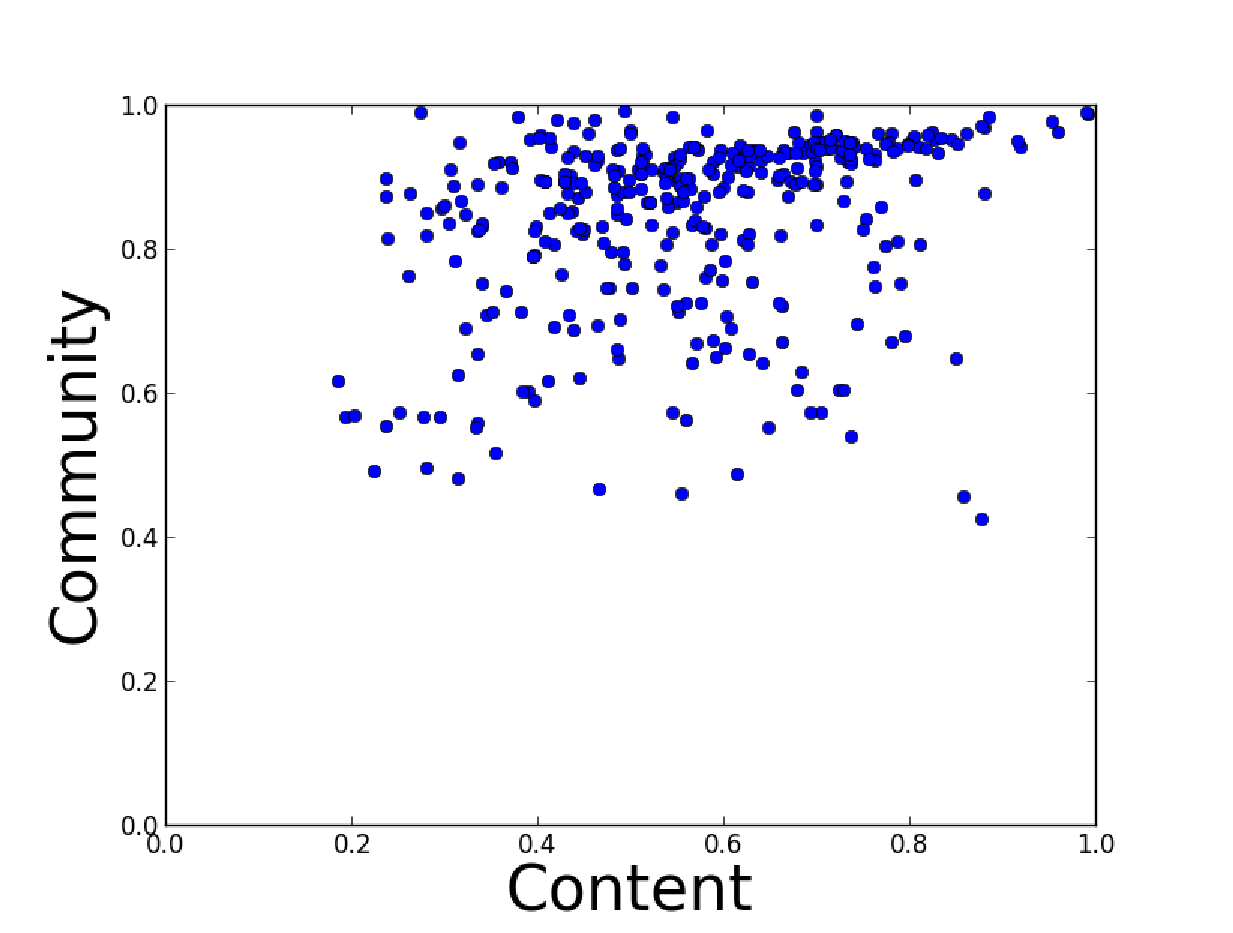
\includegraphics[width=0.5\textwidth]{KDD/images/Text-Vs-Users-sNMF-dots-new}            
\end{center}
  \caption[Stability of hashtags]{{This figure illustrates the stability of hashtags in terms of content and community information.  Each dot in the figure
is a hashtag.  The x-axis and y-axis represent content and community stability.  The content and community stability scores are 
calculated according to Algorithm \ref{alg:hashtag_stability_scores}.}  }
\label{fig:Stability}
\vspace{-0.5cm}
\end{figure}
\begin{table}
\begin{center}
\begin{minipage}[b]{1\linewidth}
{\tiny
\begin{tabular}{|lclclc|}
\multicolumn{6}{c}{\small{Twitter News Dataset}} \cr
\multicolumn{2}{c}{\bf Text-Stable} & \multicolumn{2}{c}{\bf Community-Stable} & \multicolumn{2}{c}{\bf Mixed} \cr
\#birdflu &  & \#facts &  & \#egitto3000 & \cr
\#h7n9 &  & \#celeb &  & \#hindi &  \cr
\#google &  & \#nyt &  & \#tahrir & \cr
\#football &  & \#gossip &  & \#alarabiya &  \cr
\#taxes & & \#followfriday & & \#vrwc &  \cr
\#bangladesh & & \#cbs &  & \#jan25 &  \cr
\#chinese &  & \#businessangel & & \#news &  \cr
\#climatechange &  & \#aje &  & \#rwnjalert &  \cr
\#climate &  & \#fem2 &  & \#bigtweet &  \cr
\#nkorea &  & \#opanews &  & \#business &  \cr
\#immigration &  & \#tf &  & \#india &  \cr
\#iran &  & \#interesting &  & \#smallbusiness & \cr
\#gun &  & \#top & & \#nhl &  \cr
\#lgbt &  & \#cincinnati &  & \#forbes &  \cr
\#dprk &  & \#thn24en & & \#buisnessguide &  \cr
\#nba &  & \#ihatetimwaterman &  & \#tcot &  \cr
\#japan &  & \#stopoccopywaste &  & \#financenews &  \cr
\#tax &  & \#divalishdesigns &  & \#adityaramadana & \cr
\#nuclear & & \#informate &  & \#shubhamconsultants & \cr
\#education & & \#olympic &  & \#money &  \cr
\end{tabular}
} %tiny
\centering 
\end{minipage}
\caption[A list of the top hashtags in each category.]{{This table lists the top-$20$ hashtags found in the content stable, community stable and mixed stable categories.
Basically these are closest $20$ points by Euclidean distance from $(1,0)$, $(0,1)$ and $(1,1)$ in Figure \ref{fig:Stability}
for content stable, community stable, and mixed stable hashtags respectively.  These were used as the groundtruth
for evaluating topic discovery (more details on evaluation in Section \ref{sec:experiments}).}}
\label{tab:tags}
\end{center}
\vspace{-0.8cm}
\end{table}

Recall that we use the hashtags as the groundtruth
topic of the text document.
Keeping in mind our research questions from Section \ref{sec:introduction}, we wanted to detect the three different
categories of hashtags for each dataset.
The first category of hashtags are those that are stable in terms of content, but relatively unstable in terms of community; 
meaning that the content corresponding to these hashtags does not evolve much over the period of interest, but the community
of users who tweet about these hashtags evolves quite a bit.
We call this set \emph{content stable} hashtags.  These are the supposedly `easier' topics where one may expect
that the presence of community may not particularly help in better topic discovery.
The second category of hashtags are those that are stable in terms of their community, but the content evolves a lot;
meaning that the community of users that show an interest on these tags stays relatively unchanged over a period of time,
but the actual content (in terms of vocabulary) changes a lot.
We call this set \emph{community-stable} hashtags.  These are the supposedly more difficult topics where using
the content alone may yield only poor performance, since by definition the content is not very stable.
The third category of hashtags are those that are stable in terms of both content and community, called \emph{mixed-stable}
hashtags.  
Intuitively, we posit that our model would work particularly well in discovering and monitoring those topics which 
have a stable community of active users over the period
of interest, but have a content which is evolving a lot (these are community-stable hashtags).

Following the notation specified in Section \ref{sec:content_and_networks}, we explain how we determine the 
tags which fall into the content-stable, community-stable, and mixed-stable categories.
Let us consider matrix $\mathbf{T}^{(t)}$ of size $N_h^{(t)} \times N_d^{(t)}$, 
where  $N_h^{(t)}$ is the number of hashtags produced at time $t$ and 
$N_d^{(t)}$ is the number of documents arriving at time $t$.
In particular, $\mathbf{T}^{(t)}(i,j) = 1$ if the document $j$ has been mentioned in a tweet
that contains the hashtag $i$, and $0$ otherwise.  Algorithm \ref{alg:hashtag_stability_scores} explains
how we compute a stability score for each hashtag in terms of their content and community. The essence of Algorithm
\ref{alg:hashtag_stability_scores} is as follows: by simply averaging all the documents belonging to a particular
hashtag, we obtain a representation for each hashtag in terms of features extracted from the documents. Following this procedure, each hashtag can consists of a (centroid) vector of  $N_f$ entries (i.e., in a bag-of-words representation).  We compare this representation with a similar
representation obtained for the same hashtag at the next time step using cosine similarity.  We then average
all the similarities obtained across the consecutive time steps for each hashtag.

Refer to Figure \ref{fig:Stability}.  Note that, in such a figure, the point $(1,0)$ represents perfect content stability, and zero community
stability.  To determine the set of hashtags that belong to the \emph{content stable} set, we calculate the Euclidean distance between
$(1,0)$ and all the other hashtags, and rank them in the increasing order of their distances.  Likewise for \emph{community stable} and
\emph{mixed stable} sets (using respectively the Euclidean distances to points $(0,1)$ and $(1,1)$).  
Some examples of content stable hashtags are \texttt{\#football} and \texttt{\#h7n9}; community stable hashtags,
\texttt{\#celeb} and \texttt{\#gossip} and mixed stable hashtags \texttt{\#alarabiya} and \texttt{\#forbes}.
\vspace{-0.2cm}


\section{Experiments}
\label{sec:experiments}
%!TEX root = paper.
\begin{figure*}[!t]
\begin{minipage}{0.310\linewidth}
  \centering
  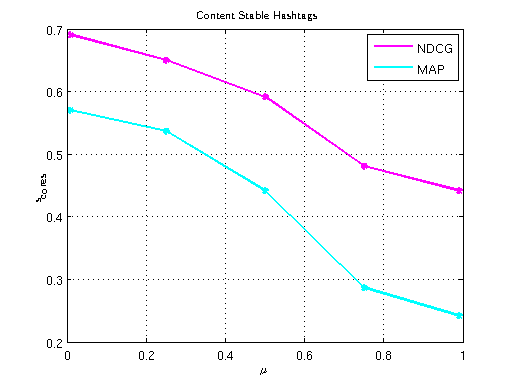
\includegraphics[width=1\textwidth]{KDD/images/content}             
   (a) content stable; $k = 5$ 
\end{minipage}
\begin{minipage}{0.310\linewidth}
  \centering
  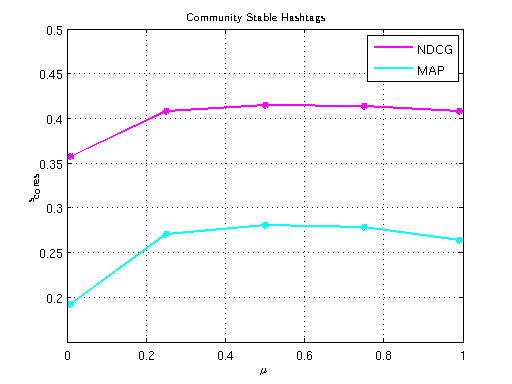
\includegraphics[width=1\textwidth]{KDD/images/community}             
  (b) community stable; $k = 5$
\end{minipage}
\begin{minipage}{0.310\linewidth}
  \centering
  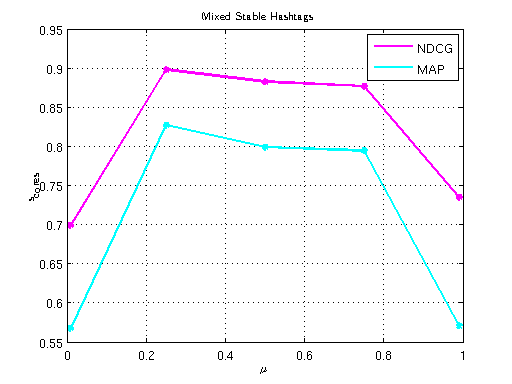
\includegraphics[width=1\textwidth]{KDD/images/mixed}             
  (c) mixed stable; $k = 5$
\end{minipage} \\
\begin{minipage}{0.310\linewidth}
  \centering
  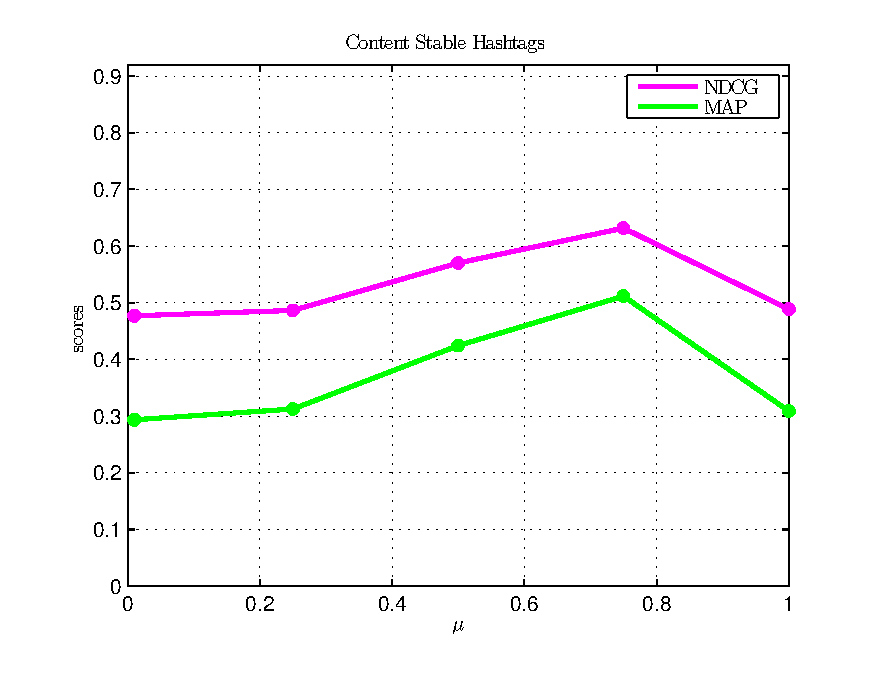
\includegraphics[width=1\textwidth]{KDD/images/content_t_15}             
   (d) content stable; $k = 15$
\end{minipage}
\begin{minipage}{0.310\linewidth}
  \centering
  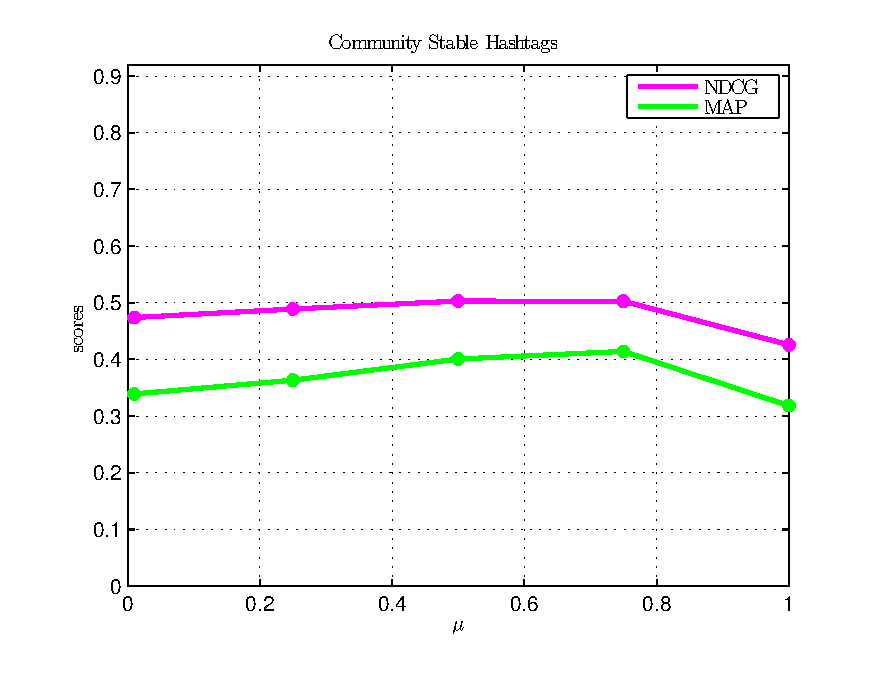
\includegraphics[width=1\textwidth]{KDD/images/community_t_15}             
  (e) community stable; $k = 15$
\end{minipage}
\begin{minipage}{0.310\linewidth}
  \centering
  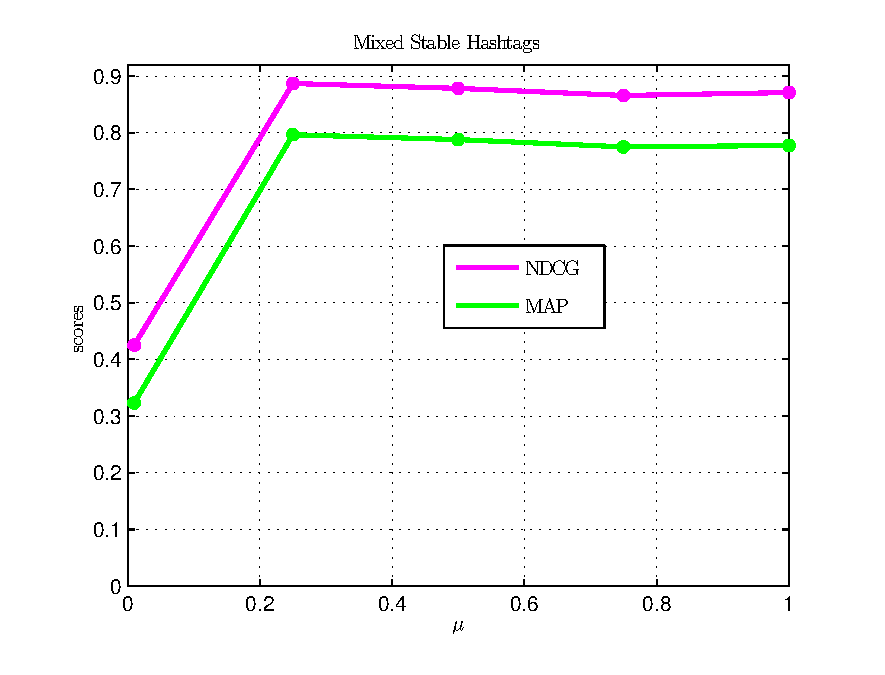
\includegraphics[width=1\textwidth]{KDD/images/mixed_t_15}             
  (f) mixed stable; $k = 15$
\end{minipage}
  \caption[Effect of $\mu$.]{{This figure illustrates the effect of the importance parameter, $\mu$ on the performance.  
Refer to Equation \ref{eq:loss_function}.  A high value of $\mu$ places more weight on the topic part of the objective
and less weight on the community part of the objective, and vice versa.
}}
\label{fig:mu_analysis}
\end{figure*}
Recall that our goal in this work is to gain a better understanding of when the
social context surrounding the documents actually improve topic discovery.
Hence, in this section, our primary focus is to provide a quantitative and 
qualitative answers to each of the research questions posed in the introduction. 
Section \ref{subsec:baselines} provides an overview about the baseline algorithms,
details how we implement them, and how we use them in our
problem setting.  Section \ref{subsec:ground_truth_evaluation}
provides details about how the groundtruth topics are obtained.  In addition,
it also explains how the topics detected by our algorithm and each of the baselines are compared with
the groundtruth  topics, and what metrics are used for the evaluations.
Then, each of the subsequent subsections are dedicated to answering one or more 
research questions.
\subsection{Baselines}
\label{subsec:baselines}
We evaluate our algorithm with several baselines.  Our baselines can be divided into two categories;
one which focuses on modeling topic evolution, and another which aims to incorporate link information
into topic modeling.

\emph{Link-PLSA-LDA} \cite{Nallapati:2008} is an algorithm which uses both the content
and link information (but does not have a temporal aspect incorporated in it). 
The link structure is built from the citation network of the documents.
The algorithm combines LDA and PLSA into a single
framework and in addition, models the topical relationship between the citing document
and the cited document.\footnote{While we do not explicitly compare to \cite{Erosheva:2004}, the
authors of Link-PLSA-LDA compare
their own work to former and claim better performance.}  The inference is carried out by
employing mean-variation approximation of the latent variables.  To implement this algorithm, 
we used the code developed by the authors which is available publicly.\footnote{\hyperref[]{https://sites.google.com/site/rameshnallapati/software}}  As input, the algorithm requires
a list of documents in a bag-of-words format, and a matrix of links between the documents.  Producing
bag-of-words for each document is straightforward.  For the link information, 
we assume that a link exists between two articles if they have a common user sharing or posting
the article.  This information was essentially derived from the $\mathbf{U}$ matrix in Section
\ref{sec:data_set_description}.  Each fresh inflow of documents is considered as a separate problem
as the model was not developed to connect topics temporally.

\emph{Collective Matrix Factorixation} (CMF) \cite{Saveski:2014, Ding:2014} 
Broadly speaking, the concept of collective matrix factorization has been
used in several applications including recommendation systems, producing hashing functions for images, co-clustering etc.
In this scenario, we will use CMF to incorporate both the social and textual aspect
of the objective in Equation \ref{eq:loss_function} but not its temporal aspect.
We compare our method to this
baseline to show that using the temporal information of tracking the textual content and community helps improve
performance.

\emph{Online-LDA} \cite{AlSumait:2008} is an algorithm which monitors topic evolution, in that it utilizes 
the information about topics detected in the previous time steps, but does not accommodate 
for the link structure between the documents.  We implemented Online-LDA based
on the original LDA code developed by David Blei\footnote{\hyperref[]{http://www.cs.princeton.edu/~blei/lda-c/}} 
(as suggested by the authors of \cite{AlSumait:2008}).  The authors
of \cite{AlSumait:2008} had found that using the topics detected in the previous time step produced the most improvement in
performance, and suggested that using the topics from earlier time steps produced only marginal improvements.  
We tested this baseline in a similar setting as well and used only the topics in the previous timestep to discover current topics.
In essense, implementing Online-LDA boils down to setting the prior on the topics according to the topic
distribution discovered in the previous time step.

\emph{Joint Past Present Decomposition} (JPP) \cite{Vaca:2014} models also the topic evolution, but as Online-LDA, is blind to the social context surrounding the  input documents.  Our method, LTECS, reduces to JPP when $\mu = 1$.
We used the code provided by the authors.\footnote{\hyperref[]{https://github.com/amantrac/TopicDiscoveryJPP}}
\subsection{Evaluation, Groundtruth and Experimental Setup}
\label{subsec:ground_truth_evaluation}
We evaluate all the algorithms by comparing a ranking of the top-$10$ words obtained by each
algorithm, and a ranking of the top-$10$ words obtained by the groundtruth.  It has been shown that
the group of top-$10$ words indeed give us a good insight about the topic \cite{sekiguchi:2006,newman2010automatic}.
All the algorithms considered here including the baselines and LTECS
discover topics by directly producing a distribution over words. 
In terms of mapping the discovered topics to the groundtruth topics, we calculated
the cosine similarity between each of the discovered topics and the groundtruth topics.
Each discovered topic was then mapped to the most similar groundtruth topic.
We borrow this procedure procedure from other state of the art experiments
in topic evolution \cite{Saha:2012}.
The distributions produced in each case are discrete and can be used 
to pick the top-$10$ words in each topic and to produce a ranking.

We now delve a bit more into how the groundtruth is obtained.  On Twitter, hashtags are a sequence of non-whitespace
characters which follow the \# sign.  It is popular convention on Twitter to embed a hashtag
in a tweet to give it context.
And as in several studies in the past, this context is used as the groundtruth topic annotations for
the news articles whose links are embedded in the tweet \cite{Tsur:2012}. 
The hashtags for each of the three categories, content stable,
community stable, and mixed stable were identified as explained in Section \ref{subsec:hashtag_stability}.

The way we calculate
the actual groundtruth topic distribution is that, 
at each time step, the $\mathbf{T}^{(t)}$
matrix (refer to Section \ref{sec:data_set_description} for notation) is premultiplied by $\mathbf{X}^{(t)}$
to obtain a resulting matrix of raw word counts for each topic.  Premultiplication of $\mathbf{T}^{(t)}$
by $\mathbf{X}^{(t)}$ basically yields the average word distribution within each hashtag.  
Once this is obtained, the highest weighted $10$ words form our groundtruth ranking.  We use
Normalized Cumulative Discounted Gain (NDCG) metric, and the Mean Average Precision (MAP) metric
to compare the rankings obtained by each algorithm to the groundtruth.  We have performed
experiments by considering the best $5,10,15 \text{ and } 20$ topics for each category.  

We now give details about the experimental setup.  Our objective function is optimized
iteratively using the multiplicative update equations (Equations \ref{eq:W_update} - \ref{eq:MC_update})
in Section \ref{sec:content_and_networks}.  The variables $\W, \HH, \G, \MT, \MC$ were given
a random non-negative initialization.  The parameters were tuned on all
the data.  In both datasets, the data spans for 14 days, and hence the topic discovery results that
we obtained are averages of the results obtained over that time period.
The $l1$ normalization parameter for CMF, the JPP model and the LTECS model were set to $0.05$.
The $\lambda$ parameter was tuned for values of $\{10, 100, 10^3 \ldots 10^7\}$.  It was consistently
observed that the algorithm yielded good performance for $\lambda = 10^7$
\footnote{While it so happens that this value of lambda worked well for the Twitter dataset, it may
not hold for other datasets.  As a matter of fact, we explore this more in Section \ref{subsec:learning_stability}
where we try to assess the quality of topics by setting $\alpha = 0.5$ and $\lambda = 0$.}.
We tuned for different values of $\mu \in \{0.01, 0.25, 0.5, 0.75, 1\}$ and picked the one which gives the best performance.
We delve more into the analysis for $\mu$ in subsequent sections.  For the baselines, all the parameters
were tuned and set internally.
\subsection{Social Information Vs Textual Content: the Trade-off}
\label{subsec:parameter_analysis}
The $\mu$ parameter from Equation \ref{eq:loss_function} allows to
bias the objective function more
towards one of the modalities, if so desired.  A high value of $\mu$ biases importance to the content part of
the objective and vice versa.  In fact, LTECS reduces to JPP when $\mu = 1$ and hence JPP can never
outperform LTECS.  This section delves into investigating how the trade-off between using content and social information
actually functions on both datasets. 

For the case of \emph{community stable} hashtags, the best performances
were achieved for $0.01 \leq \mu \leq 0.5$ (Table \ref{tab:topic_discovery_evaluation}).
This implies that when a lot of importance was placed on the social context part
of the objective, better were the topics that were detected. Refer to Figure \ref{fig:mu_analysis}b
and \ref{fig:mu_analysis}e.  These figures illustrate how the performance varies as the value of $\mu$
moves from $0$ to $1$.  Note that highest performance is achieved when $\mu \leq 0.5$.

While considering \emph{content stable} hashtags, we will focus on LTECS and JPP
in Table \ref{tab:topic_discovery_evaluation}. For $k = 5 \text{ and } 10$, we observe best
performances by \emph{both} JPP and LTECS method.  In other words, LTECS
algorithm exhibited best performance when the objective contained only the content part with $\mu = 1$.  
This suggests that for topics which have a highly focused text, we need to place all the 
importance on content.  What is more interesting is that, it implies that even if we add a little
bit of the social context information to the objective, it actually \emph{hurts} performance.
Let us contrast this result to what happens when $k = 15 \text{ and } 20$.
In those scenarios, we observe that the best performance was
obtained by LTECS, when $\mu$ was $0.75$.  
For the purest $5$ and $10$ topics, it could be that the content of those documents 
were very well defined that the usage of side information actually detracted the objective 
from the correct path.  However as the number of topics
increases ($k = 15, 20$), there is perhaps more noise in the topics and
we find that the use of community information indeed helps.  
This suggests that for the best performance one needs to know the accurate
operating spot of the $\mu$ parameter.  
The important message from analyzing the $\mu$ trade-off for content stable and community
stable hashtags is that, with very focused text, just using the content suffices. This is likely to be the case for the dominant topics (i.e. $k<10$ in our study).
On the other hand, if the text is a little noisy, the social context greatly
helps in discovering better topics. 
This is likely to be the case when tracking more than just the top dominant topics ($k>10$ in our case).  
As we argue in the introduction, in today's world,
the text is more often than not quite noisy as topics are prone to being volatile and evolving
very quickly.  Refer to Figures \ref{fig:mu_analysis}(a) and \ref{fig:mu_analysis}(d).  The figure
illustrates that the best performance is acheived when $\mu \geq 0.5$.

By definition \emph{mixed stable} hashtags have both stable content and stable communities.  
As it turns out, the best performance for LTECS is obtained when $0.25 \leq \mu \leq 0.75$.
This suggests that when we have topics which have both stable content and community,
it is necessary to give importance to both aspects.  In addition, biasing only on content
does not yield the best performance.  In Figures \ref{fig:mu_analysis}(c) and \ref{fig:mu_analysis}(f),
the best performance is achieved in the midregion of the plot.
\subsection{Comparison with the state-of-the-art}
\label{subsec:topic_discovery_experiments}
In this section, we discuss how our algorithm performs in 
comparison to state of the art baselines introduced in Section \ref{subsec:baselines}.
One of the main conclusions from analyzing the results is that, using the community
information certainly helps with better topic tracking.  This is a direct observation
from Table \ref{tab:topic_discovery_evaluation} that the NDCG and MAP values for LTECS
is higher, or at least as good as its competitors in most scenarios.  The rest of this section
will highlight where the sweet spot of the trade off between content and community
lies, and why.

For \emph{community stable topics}, as expected, good improvements were seen in the community stable hashtags.  In these hashtags,
LTECS algorithm consistently outperforms all the baselines.  It is clear that
the use of community information helps in better topic discovery.  It is also interesting
to note that the algorithm that exhibits second best performance is Link-PLSA-LDA.  
Hence, not learning from older topics does not particularly hurt Link-PLSA-LDA
in its performance when compared to Online-LDA and JPP.  This means that, for community stable topics, 
the algorithms that use some form
of social context information or link information perform better than those that discover topics using
content alone.

In the case of \emph{content stable topics}, one may expect the baselines which focus only
on the content of the documents to exhibit best performance.  This is partially true.  For $k = 5,10$,
JPP and LTECS outperform Link-PLSA-LDA and Online-LDA.  Note that in both cases
LTECS achieves the best performance only when $\mu = 1$ implying that adding community information
does not help.  On the other hand, for $k = 15 \text{ and } 20$, LTECS achieves best performance
over all the baselines.  In these cases note that the value for $\mu = 0.75$.  This implies
that adding the community information actually helps.  We already discussed this behavior in Section \ref{subsec:parameter_analysis}.
 Another thing to note here is that Link-PLSA-LDA some what consistently ranks last.  This is because
Link-PLSA-LDA, unlike LTECS lacks the tuning parameter $\mu$ which can seamlessly shift the focus of the
objective between topic and community.  It perhaps places equal weight on both, and hence fails to
make the appropriate tradeoff.

For \emph{mixed stable hashtags}, the performance is in generally very good for all the hashtags.
This becomes clear when we compare the performance metrics of content stable and community stable to mixed stable.  There
is a noticeable jump in the average NDCG and MAP scores.  This implies that, if a hashtag
has both well focused content, and a dedicated community of users, detecting those topics
are much easier. 
\begin{table*}[!t]
\begin{center}
{\small 
{\renewcommand{\arraystretch}{0.91}
\begin{tabular}{||c|c|c|cccc||}
\hline
 Category of Topic &Metric & Model & k = 5 & k = 10 & k = 15 & k = 20\\
\hline
 		    & & LTECS & 0.4081 & \textbf{0.4800} & \textbf{0.5029} & 0.5129\\
Community 	& &  & $\mu =  0.01$  & $\mu = 0.5$ & $\mu =  0.5 $ & $\mu = 0.5$\\ \cline{4-7}	
		    & NDCG & JPP & 0.3699 & 0.4496 & 0.4608 &0.4138\\
			&  & Online-LDA & 0.3903 & 0.4138 &0.4446  & 0.5667 \\
Stable       & & Link-PLSA-LDA &0.3943 & 0.4608 & 0.4761 & 0.4925\\ 
        & & CMF & 0.3454 & 0.4338 & 0.4771 & 0.4827 \\ \cline{4-7}
		& & LTECS & 0.2653 & 0.3637 & \textbf{0.4007} & \textbf{0.4173}  \\
		& &  &$\mu = 0.01$ & $\mu = 0.5 $ & $\mu = 0.5$  & $\mu = 0.5$ \\ \cline{4-7}
Hashtags&MAP & JPP &  0.2191 & 0.3596 & 0.3462 & 0.3420 \\
		& & Online-LDA & 0.2628  & 0.3160 & 0.3489 & 0.3835 \\
		& & Link-PLSA-LDA & 0.2704 & 0.3364  & 0.3658 & 0.3937 \\
        & & CMF & 0.2044 & 0.3190 & 0.3757 & 0.3665 \\
\hline
		& & LTECS &\ 0.6888 & 0.6055& \textbf{0.6317}& \textbf{0.6623} \\
Content   & &  & $\mu =  1$  & $\mu = 1$ & $\mu =  0.75 $ & $\mu = 0.75$\\ \cline{4-7}
		&NDCG & JPP & 0.6888 & 0.6055 &  0.4885&  0.6504 \\
		& & Online-LDA & 0.6815& 0.5988 & 0.6166 & 0.6684  \\
Stable  & & Link-PLSA-LDA & 0.6574 & 0.5862 & 0.6087& 0.6401\\ 
        & & CMF & 0.5846 & 0.4919 & 0.4455 & 0.4327 \\\cline{2-7}
		& & LTECS & \textbf{0.5655} &  \textbf{0.4784}& \textbf{0.5115} & \textbf{0.5559}  \\
		& &  & $\mu =  1$  & $\mu = 1$ & $\mu =  0.75$ & $\mu = 0.75$\\ \cline{4-7}
Hashtags &MAP & JPP &  0.5655 & 0.4784 & 0.3089 & 0.5411  \\
		& & Online-LDA &  0.5175 & 0.4083 & 0.4555 & 0.5443 \\
		& & Link-PLSA-LDA & 0.4890 & 0.3817  &0.4434 &0.5053  \\
        & & CMF & 0.4423 & 0.3207 & 0.2556 & 0.2557 \\
\hline
	    & & LTECS & 0.9005 & 0.8868& \textbf{0.9249}& 0.9089 \\
Mixed   & &  & $\mu =  0.25$  & $\mu = 0.75$ & $\mu =  0.25 $ & $\mu = 0.25$ \\ \cline{4-7}
		&NDCG & JPP & 0.8771 & 0.8762 & 0.4251 & 0.4580 \\ 
	    & & Online-LDA &\textbf{0.9564} & 0.9168 & 0.9111 & 0.5967 \\
Stable  & & Link-PLSA-LDA & 0.8944 & 0.9159 &0.8392 & 0.8975 \\ 
        & & CMF & 0.6712 & 0.8768 & 0.8905 & 0.8753 \\ \cline{2-7}
		& & LTECS & 0.7783 &0.7965  & \textbf{0.8964} & 0.8845 \\
		& &  & $\mu =  0.25$  & $\mu = 0.75$ & $\mu =  0.5$ & $\mu = 0.25$ \\ \cline{4-7}
Hashtags&MAP & JPP &  0.7762 & 0. 7783 & 0.3232 & 0.3644  \\ 
		& & Online-LDA & \textbf{0.9208}  & \textbf{0.8804} & 0.8841 & 0.4308 \\
		& & Link-PLSA-LDA & 0.8787 & 0.8379  & 0.7452 & \textbf{0.8982} \\
        & & CMF & 0.5329 & 0.8223 & 0.8499 & 0.8337 \\
\hline
\end{tabular}
}
}
\caption[Evaluation of topic discovery]{{Topic discovery evaluation using Normalized Cumulative Discounted Gain and Mean Average Precision metrics
for all three categories of hashtags.  $k$ stands for the number of topics.  $\lambda$ was set to $10^7$, and $\alpha$ was set to 0.05 for LTECS model.
All the values in bold represent significant improvement in performance (using Student-t test, $p < 0.05$).}}
\label{tab:topic_discovery_evaluation}
\end{center}
\end{table*}
\subsection{Learning Stability of Topics}
\label{subsec:learning_stability}
In this section, we investigate to what extent can our algorithm learn the type of
topics present in the documents; i.e., are the documents more content stable,
community stable or mixed stable. And we certainly do not want to be able to bias the
objective function more towards one of the modalities.  Hence, for all experiments
in this section, we set $\mu = 0.5$.
Recall that our loss function (Equation \ref{eq:loss_function}) is built such
that $\HH \approx \mathbf{M} \Htt$. 
The proposed model encourages for stability of topics and communities by regularizing the evolution matrices 
$\MT$ and $\MC$
through $\lambda(||\MT - \I||_F^{2} + ||\MC - \I||_F^2)$. 
A high value of $\lambda$ pushes the evolution matrices close to $\mathbf{I}$ 
which enforces the topics (and communities) to evolve very little over time.  
So far, we demonstrated the effectiveness of using side social information in 
order to discover topics on large scale dataset based on Twitter.
In this section, we aim to assess the extent to which our 
algorithm is able to recover correctly the evolution patterns exhibited by 
the data by studying the evolution matrices $\MT$ and $\MC$ across consecutive time steps.

This raises the question of how to set $\lambda$. In presence of a groundtruth this parameter 
can be tuned by cross validation as we did in the previous section (where hashtags where used as proxy 
to build the groundtruth). However, in the real world, topical annotations are rarely available. 
In this context, the user can decide to use the model in an ``agnostic mode" by not placing 
any form of prior on the evolution matrices. 
This is achieved by setting $\lambda$ to 0.  In this real world scenario, we may wonder if the model, 
without the help of any prior, will be able to recover the correct evolution patterns. In other words, we 
propose to test the extent to which the retrieved evolution matrices are close to the ``real ones". To do so, 
we make use of the group of hashtags previously identified (Section \ref{sec:data_set_description}) as 
stable and unstable at the topic and community level. To validate that the retrieved $\mathbf{M}$ 
matrices exhibit a temporal stability pattern which is indeed present in the data, we test if the matrix retrieved 
from the stable group of hashtags is closer to the identity than the one retrieved from 
the unstable group (for both topics and communities).  In other words, for topic stable hashtags,
we want $\MT$ to exhibit more stability than $\MC$ and for community stable hashtags,
we want $\MC$ to exhibit more stability than $\MT$.
 
For the purpose of the experiments, we need to measure how close an evolution matrix 
$\mathbf{M}$ is to the identity $\mathbf{I}$.  Or, in other words how stable is the 
evolution exhibited by $\mathbf{M}$.  Now, we will quantify this closeness.
An important point to remember now is that, many distance or similarity measures will fail to capture
the notion that we are after.  For example, quantifying the stability of $\mathbf{M}$ by simply 
calculating a cosine similarity between $\mathbf{M}$ and $\mathbf{I}$ will not work because $\mathbf{M}$
is prone to topical (and community) permutations over time.  Since we are working in an unsupervised setting,
what was `topic-1' at time-$t$ could have been discovered as `topic-5' at time-$(t+1)$.  Hence, we must
make sure that the resulting definition of stability is invariant to such topical (and community) permutations.

To quantify stability, first note that, through the primal feasibility conditions (Equation \ref{eq:primal_feasibility}), we have
$\MT \geq \textbf{0}$, and $\MC \geq \textbf{0}$.  Therefore, when we apply $l1$ normalization to the row or
column of the $\mathbf{M}$ matrices, we obtain stochastic matrices.   Also, recall that the largest eigenvalue 
of a stochastic matrix is $1$.  We now define the stability score for the evolution matrix $\mathbf{M}$ as follows:
\begin{definition}
Let $M$ be a stochastic matrix obtained after $l1$ normalization of the evolution matrix $\mathbf{M}$.  The \emph{stability} of $M$ is defined as:
\begin{equation}
\text{stability}(M) := \frac{\sum_i abs(\gamma_i)}{n},
\end{equation}
where $\{\gamma_i\}$s are the eigenvalues of  $M$, and $n$ is the number of rows (and of columns) of $M$.
\label{defn:stability}
\end{definition}

We make some observations about this definition.  The $stability(M)$ takes value
between $\big[0,1\big]$, since none of the individual $abs(\gamma_i)$s can exceed
1.  The matrix representing perfect 
stability would be $\I$ or a permutation of $\I$ 
(due to possible topical shifts between two consecutive time steps). 
A matrix $M$ has $stability(M) = 1 \iff$ $M = \I$ or a permutation of $\I$.  
%Amin: Not clear what the + of this sentence
%This makes
%sense, because we think of $\I$ or a permutation of $\I$ as being perfectly stable.  A higher
%stability score clearly means more stability over time.

%We perform topic discovery and tracking experiments again, but not with the intent of
%obtaining the best topic discovery and tracking performance.  This time, the aim is to
%let the system wander in an exploratory mode, and to optimize for the best $\MT$ and $\MC$
%by itself without worrying about the terms $\lambda(||\MT - \I||_F^{2} + ||\MC - \I||_F^2)$.
%Therefore, all the experiments in this section were performed by setting $\lambda = 0$ 
%(we place no regularization on $\MC$ or
%$\MT$, and we hope to learn it from the algorithm), 
%and $\mu  = 0.5$ (we are agnostic to the mode of stability of the input; i.e., whether it is
%content stable, community stable or mixed stable).

Through Definition \ref{defn:stability}, we investigate if the model can recover the
temporal topic and community stability patterns.  We evaluate this for each category of hashtags
by calculating the $\text{stability}(M)$
for the $\MT$ and $\MC$ calculated in each time step, and producing an average value.
$stability(M)$ is calculated through two ways: by calculating the left and right
eigen values of the $\mathbf{M}$ matrices.
We confirm that the model can recover a more stable temporal matrix for topics than for 
communities when processing hashtags with topical stability (Figure \ref{fig:stability_analysis}, left).  
While when processing hashtags that are community stable, the model recovers a more stable temporal 
community matrix (Figure \ref{fig:stability_analysis}, right).  We are thereby able to
see that using such stability analysis of the evolution matrices, one can study the nature
of the text corpora when there is no prior knowledge.  This will actually help the user
determine a value for $\mu$.
\begin{figure*}[!t]
\begin{center}
{\small
\begin{minipage}{0.49\linewidth}
  \centering
  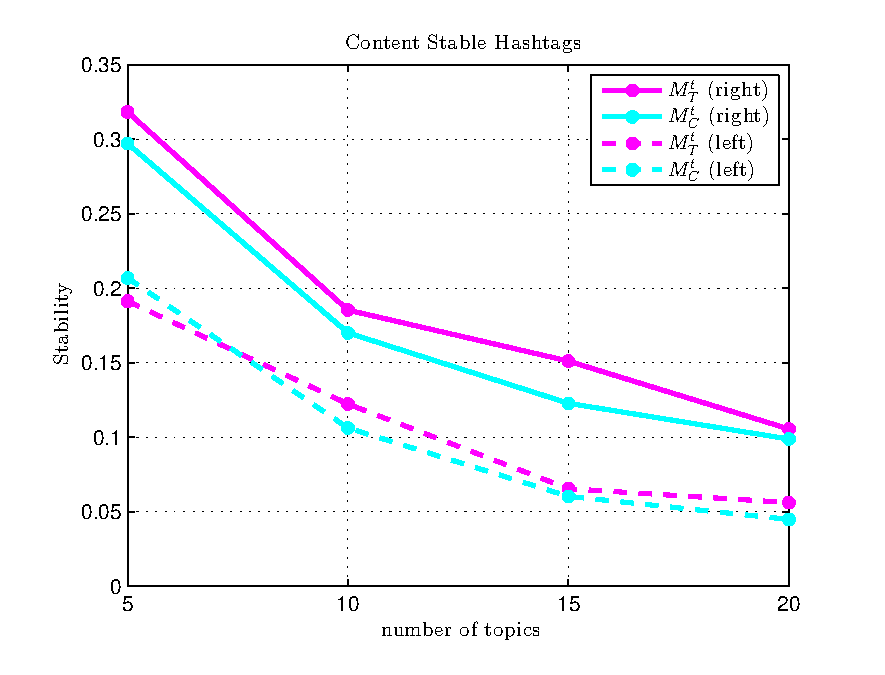
\includegraphics[width=\textwidth]{KDD/images/content_stable_eigen_left_right}          
	%{\tiny(a) Content Stable }
\end{minipage} 
\begin{minipage}{0.49\linewidth}
  \centering
  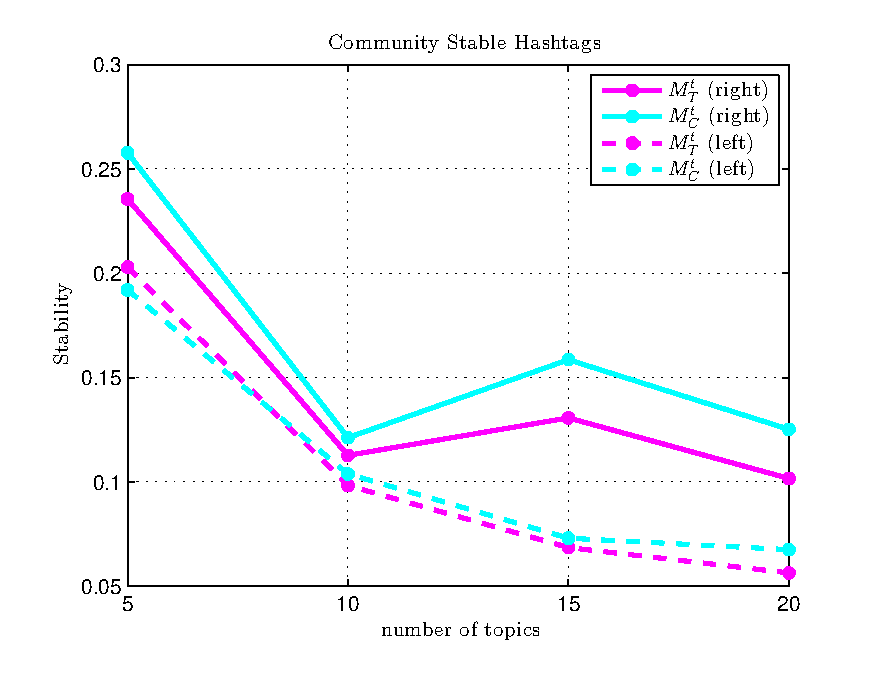
\includegraphics[width=\textwidth]{KDD/images/community_stable_eigen_left_right}             
	%{\tiny(b) Community Stable}
\end{minipage} 
  \caption[Stability of evolution matrices]{{This figure plots the stability of $\MC$ and $\MT$.
We note that in (a) $\MT$ matrix shows higher stability than the $\MC$ matrix,
and in (b) $\MC$ shows higher stability than $\MC$, thus confirming that we are indeed able to learn the 
stability through our algorithm.}}
  \label{fig:stability_analysis}
}
\end{center}
\end{figure*}


\section{Conclusion}
\label{sec:conclusion}
The goal of our work was to gain a better understanding of when social context
helps in modeling topic evolution.  In order to achieve this, we proposed a matrix factorization based
approach which takes into account both the content of the documents and their social
context.  We found that, depending on the kind of topic, there is a clear trade
off between the content and community.
The content of the document
suffices if the text of the topic is very focused, and evolves little over time.
As we begin to move away from this scenario to consider documents that have a richer
and more variable vocabulary, we find that the use of social context
begins to help greatly.  We were also able to show
that our model can learn the kind of topics at hand; i.e., whether they are
content stable, community stable, or
both.

This work predominantly considered the user interactions of the documents
as the social context.  In the same spirit, one could explore what it means to consider
other types of contexts like geographical location of the user (or document),
and also perhaps delve more into the user profiles and incorporate information
about age, gender and demographics to give a well rounded view of the social context.
We hope to be able to work on these aspects in the future.
 
\chapter{Prediction and Characterization of High-Activity Events
in Social Media}
\label{plos_chapter}
On-line social networks publish information on a high volume of
real-world events almost instantly, becoming a primary source for
breaking news.  Some of these real-world events can end up
having a very strong impact on on-line social networks.  The effect of such
events can be analyzed from several perspectives, one of them being
the intensity and characteristics of the collective activity that it
produces in the social platform.
We research 5,234 real-world news events encompassing 43 million
messages discussed on the Twitter microblogging service for
approximately 1 year.  We show empirically that exogenous news events
naturally create
collective patterns of bursty behavior in combination with long periods of
inactivity in the network. This type of behavior agrees with
other patterns previously observed in other types of natural collective phenomena, as
well as in individual human communications. In addition, we propose a methodology to
classify news events according to the different levels of intensity in
activity that they produce. In particular, we analyze the most
highly active events and 
observe a consistent and strikingly different collective reaction
from users when they are exposed to such events.  This reaction is
independent of an event's reach and scope.  We further observe that
extremely high-activity events have characteristics that are quite distinguishable
at the beginning stages of their outbreak.  This allows us to predict
with high precision, the top 8\% of events that will have the most
impact in the social network by just using the first 5\% of the information of an
event's lifetime evolution. This strongly implies that high-activity events
are naturally prioritized collectively by the social network, engaging users early
on, way before they are brought to the mainstream audience.


\section{Introduction}

% Motivation
Social media is now a primary source of breaking news information
for millions of users all over the world \cite{Kwak:2010}. On-line
social networks along with mobile internet devices have crowdsourced
the task of disseminating real-time information. As a result, both
news media and news consumers have become inundated with much more
information than they can process. One possible way of handling this data overload, is
to find ways to filter and prioritize information that has the
potential of creating a strong collective impact. Understanding and
quickly identifying the type of reaction that certain exogenous events will produce
in on-line social networks, at both global and local scales, can help
in the understanding of collective human behavior, as well as
improve information delivery, journalistic coverage and
crisis management, among other things. We
address this challenge by analyzing the properties of real-world news
events in on-line social networks, showing that they corroborate patterns
previously identified in other case studies of human communications. In
addition, we present our main findings of how news events that produce
extremely high-activity can be clearly identified in the early stages of
their outbreak.

% Brief background on the problem

The study of information propagation on the Web has sparked tremendous
interest in recent years. Current literature on the subject primarily
considers the process through which a {\em meme}, usually a piece of
media (like a video, an image, or a specific Web article), gains
popularity
\cite{Castillo:2014,Szabo:2010,Lerman:2010,Tatar2014,Pinto:2013,Ahmed:2013,Li:2016:concept:drift,
Liu:2015:UN}.  
However, a meme represents a
simple information unit and its propagation behavior does not necessarily
correspond to that of more complex information such as
news events. News events are usually diffused in the network in many
different formats, e.g., a particular news story such as an {\em
  earthquake in Japan} can be communicated through images, URLs,
tweets, videos, etc. Therefore, current research can benefit from analyzing
the effects of more high-level forms of information. 

Traditionally, the impact of information in on-line social networks has been
measured in relation to the total amount of attention that this subject receives
\cite{berger2012makes,iribarren2011branching,guerini2011exploring,mills2012virality,gaugaz2012predicting}.
That is, if a content posted in the network receives
votes/comments/shares above a certain threshold it is usually deemed as {\em viral} or
{\em popular}. Nevertheless, this
notion of popularity or impact will favor only information that produces very large
volumes of social media messages. 
Naturally, global breaking news that has world-wide coverage and that produces a high volume of
activity in a short time should be considered as
having a strong impact on the network.  However, there are other types of events
that can produce a similar reaction in smaller on-line communities
such as, for example, on users from a particular country
(e.g., the
withdrawal of the main right wing presidential candidate in Chile due
to psychiatric problems, just before
elections \cite{chile_elections}).
Clearly, events of local scope do not produce as much social media
activity as events of global scope, but they can create a strong and
immediate reaction from users in local networks \cite{ReisBOPKA15}. Conversely,
there are large events which do not produce an intense reaction, such as
{\em The Oscars} (Fig~\ref{fig:fig1}), which span a long
period of time and are discussed by social network users for weeks or
even months, but do not spark intense user activity. Therefore, it is reasonable to consider additional dimensions,
than just volume, when analyzing the impact of information in on-line communities.  

Prior research has shown that certain types of individual activities,
such as communications (studied in email exchanges), work patterns and
entertainment, follow a behavior of bursts of rapidly occurring
actions followed by long periods of inactivity
\cite{barabasi2005origin}, referred to as {temporally inhomogeneous}
behavior \cite{karsai2012universal}.  This type of behavior initially
observed in individual activities, has also been observed in relation
to other naturally occurring types of collective phenomena in human
dynamics similar to processes seen in self-organized criticality
\cite{karsai2012universal}.  In particular, extremely high-activity
bursty behavior seems to also occur in critical situations, observed
from the information flow in cell phone networks during
emergencies\cite{gao2014quantifying}.  Although, there is research
towards modeling this type of collective behavior
\cite{yan2013information} in on-line social networks, to the best of
our knowledge, it has not yet been analyzed quantitatively.


Our work focuses on high-activity events in social media produced by
real-world news, with the following contributions:
\begin{enumerate}

\item We introduce a methodology for modeling and classifying
events in social media, based on the intensity of the activity that they
produce. This methodology is independent of the size and scope of the event,
and is an indicator of the impact that the event information had on the social network.

\item We show empirically that real-world news events produce collective
patterns of bursty behavior in the social network, in combination with long periods of
inactivity. Furthermore, we identify events for which most of their activity
is concentrated into very high-activity periods, we call these events {\em
high-activity events}.

\item We determine the existence of unique characteristics that
differentiate how high-activity events propagate in the social network.

\item We show that an important portion of high-activity events can be
predicted very early in their lifecycle, indicating that this type
of information is spontaneously identified and filtered collectively, early
on, by social network users.

\end{enumerate}
\section{Materials and Methods}

% model
We define an event as a conglomerate of information that encompasses
all of the social media content related to a real-world news
occurrence. Using this specification, which considers an event as a
complex unit of information, we study the type of collective reaction
produced by the event on the social network. In particular, we analyze 
the intensity or immediacy of the social network's response. 
By analyzing the levels of intensity in activity induced by different exogenous
events to the network, we are implicitly studying the priority that has been
collectively assigned to the event by groups of
independent individuals \cite{barabasi2005origin, karsai2012universal}. 

We characterize an event's discrete activity dynamics by using
\emph{interarrival times} between consecutive social media messages
within an event (e.g., $d_i = t_{i+1}-t_i$, where $d_i$ denotes the
interarrival time between two consecutive social media messages $i$
and $i+1$ that arrived in moments $t_i$ and $t_{i+1}$, respectively).


We introduce a novel vectorial representation based on a {\em vector
quantization of the interarrival time distribution}, which we call 
{\em ``VQ-event model''}. This model is
designed to filter events based on the distribution of the
interarrival times between consecutive messages.  This approach is inspired
by the {\em codebook-based representation} from the field of multimedia
content
analysis, which has been used in audio processing and computer vision
~\cite{ff,Vaizman}.  In our proposed approach, our method learns a set of
the most
representative interarrival times from a large training corpus of events;
each one of the representative interarrival times is known as a
{\em codeword} and the complete learned set is known as the {\em
codebook}~\cite{Vaizman}.  
Each event is then modeled using a vector quantization (VQ) that
converts the interarrival times of an event into a discrete set of values,
each value corresponding to the closest codeword in the codebook (details
in supplementary material).  The resulting VQ-event model is then a
vector in which each dimension contains the percentage of interarrival times
of the event that were assigned a particular codeword in the codebook.


The VQ-event representation is relative to an event's overall size
since the model is normalized with respect to the number of messages in the
event. Therefore the only criteria that are considered in the model are the
interarrival times of each particular event. This model allows us to group events based on the
{\em similarity of the distribution} of their interarrival times.
In those terms, we consider as high-activity events those events for which
the distribution of interarrival times is most heavily
skewed towards the smallest possible interval, zero.  In other words,
events for which the overall activity is extremely intense in comparison
with other events.

To illustrate events with different levels of intensity in activity we
present two examples taken from our analysis of Twitter data. These
examples show the interarrival time histograms for the entire lifecycle of
the two events. In
the first example, the majority of the messages about
the death of political leader Nelson Mandela
(Fig~\ref{fig:fig1}) arrive within almost zero seconds of
each other. On the contrary, the messages about The Oscars
(Fig~\ref{fig:fig1}) are much more spread out in time.
%\begin{figure}[!htb]
%  \centering
%  \begin{subfigure}{\textwidth}
%%    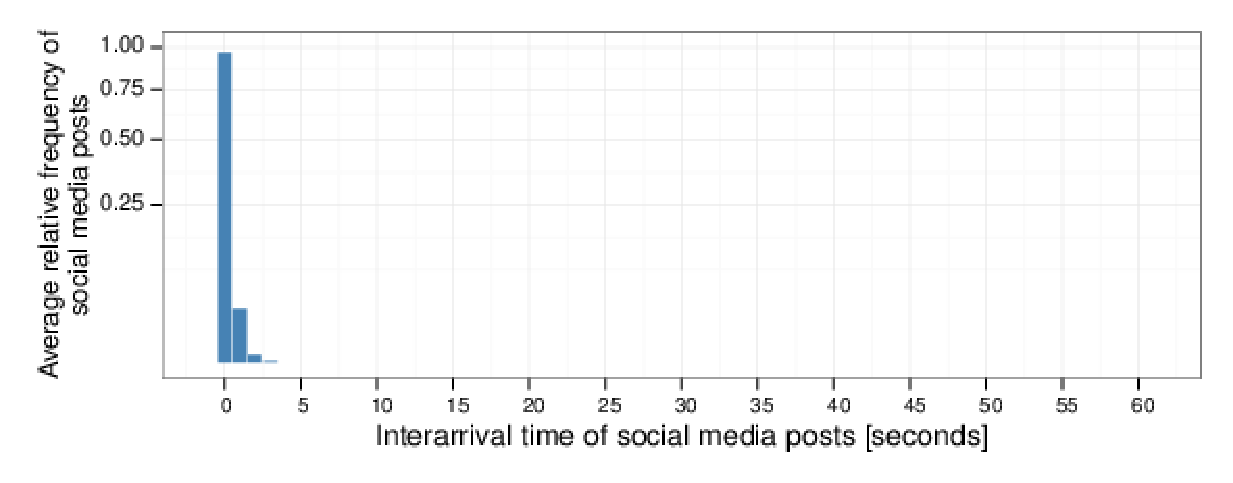
\includegraphics[width=\textwidth]{figures/plots_revision/fig1a}
%    \caption{User posts about the death of Nelson Mandela arrive
%      almost instantly.}
%    \label{fig:fig1a}
%  \end{subfigure}%
%
%  ~ %add desired spacing between images, e. g. ~, \quad, \qquad, \hfill etc.
%  % (or a blank line to force the subfigure onto a new line)
%  \begin{subfigure}{\textwidth}
%%    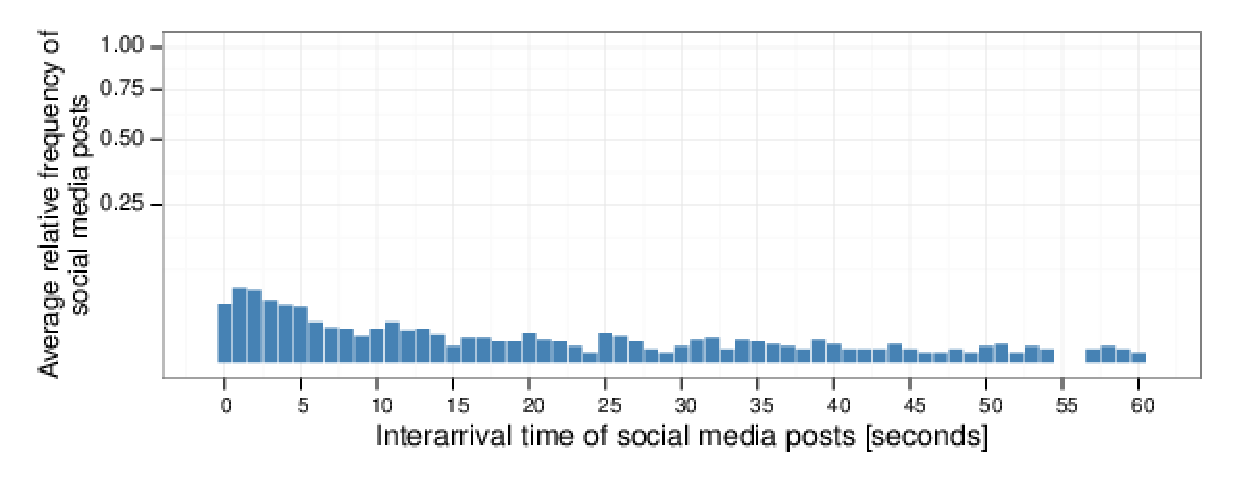
\includegraphics[width=\textwidth]{figures/plots_revision/fig1b}
%    \caption{User posts about The Oscars arriving several weeks before
%      the event.}
%    \label{fig:fig1b}
%  \end{subfigure}%
%  ~ %add desired spacing between images, e. g. ~, \quad, \qquad, \hfill etc.
%  % (or a blank line to force the subfigure onto a new line)
%
%  \caption{\textbf{Examples of interarrival time histograms of two real-world news
%events discussed on Twitter. The event [nelson, mandela] (Fig~\ref{fig:fig1a}) was
%      collected on 12/05/2013. Since there is a high
%      concentration in the first histogram bin, we conclude that most of the social media posts
%      for this event occur in one or more successions of high-activity
%      bursts (therefore, considered a high-activity event).
%      The second event, [may, oscar] (Fig~\ref{fig:fig1b}) was collected
%      on 03/23/2014 about The Oscars event that was held a few
%      weeks before. The arrival times of these posts are much more spread
%      out, displaying much less concentration of bursty activity.} 
%  }
%  \label{fig:fig1}
%\end{figure}
%
\begin{figure}[!htb]
  \centering
    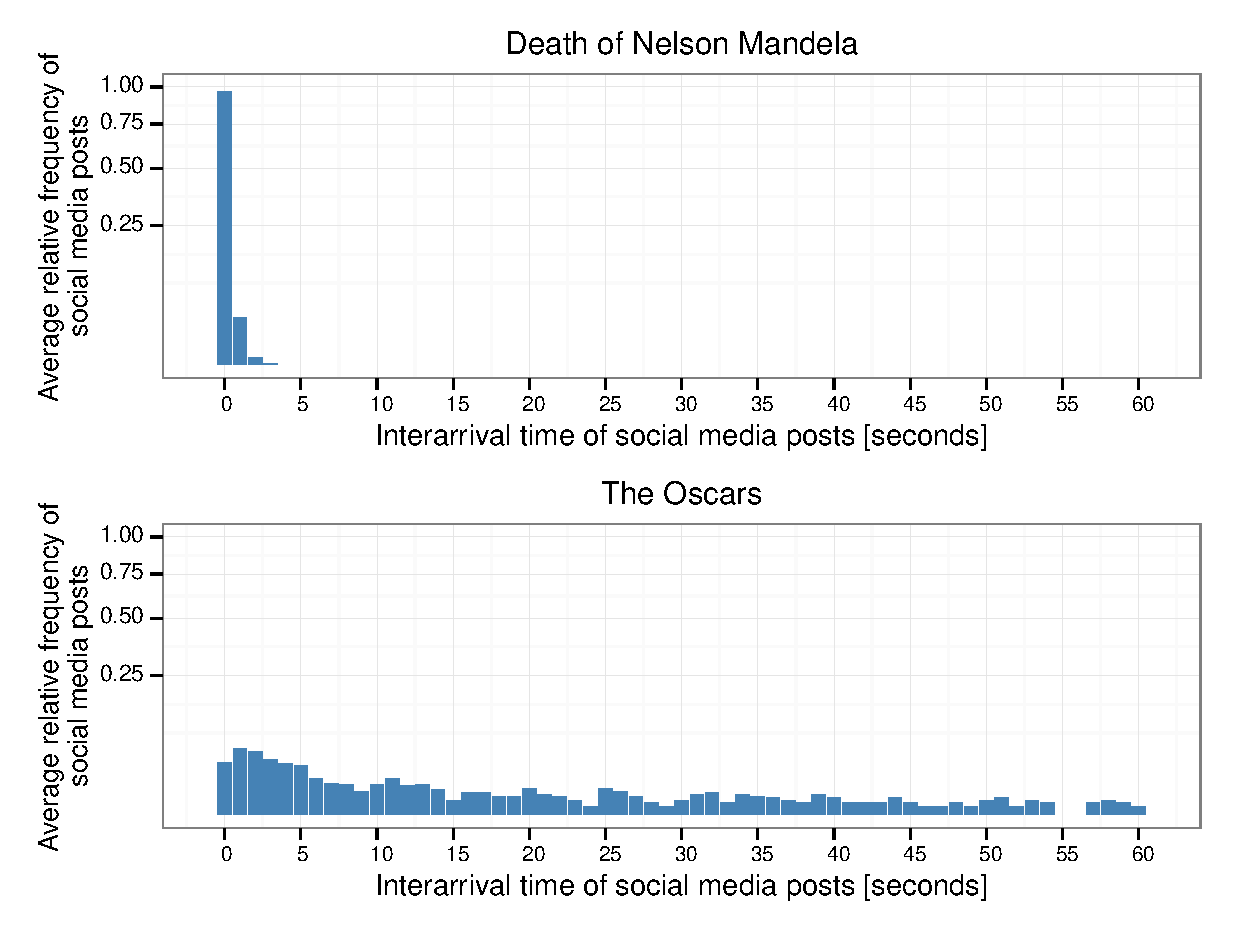
\includegraphics[width=\textwidth]{PLOSONE/figures/plots_revision/fig1}
  \caption[Examples of interarrival time histograms]{{Examples of interarrival time histograms of two real-world news
events discussed on Twitter. The event [nelson, mandela] (top) was
      collected on 12/05/2013. Since there is a high
      concentration in the first histogram bin, we conclude that most of the social media posts
      for this event occur in one or more successions of high-activity
      bursts (therefore, considered a high-activity event).
      The second event, [may, oscar] (bottom) was collected
      on 03/23/2014 about The Oscars event that was held a few
      weeks before. The arrival times of these posts are much more spread
      out, displaying much less concentration of bursty activity.} 
  }
  \label{fig:fig1}
\end{figure}


We note that, by using interarrival times to describe the intensity of the
activity of an event, we make our analysis independent of the particular
evolution of each event. By doing this, we put no restrictions on how
high-activity events unfold in time, for example, they could be: (a) events
that start out slowly and
suddenly gain momentum, (b) events that go viral soon after they appear on
social media and then decay in intensity over a long (or short) period of
time, (c) events that from the beginning produce large amounts of interest and
sustain that interest throughout their long (or short) lifespan, or (d)
events that are a concatenation of any of the above, etc.

%\newtext{ 
% Experimental analysis

We study a dataset of news events gathered from news
headlines from a \emph{manually curated} list of well-known news media
accounts (e.g., @CNN, @BreakingNews, @BBCNews, etc.) in the
microblogging platform Twitter \cite{Twitter_website}
%\footnote{\url{https://twitter.com}
%  (Accessed: August 25, 2015.)} 
(a full list of all the news media
accounts is provided in the supplementary material). Headlines were
collected periodically every hour, over the course of approximately
one year. In parallel, all the Twitter messages (called \emph{tweets})
were extracted for each news event using the public
API \cite{Twitter_API}.
%\footnote{\url{https://dev.twitter.com/} (Accessed: August 25,
%  2015.)},
% In this research, since we focus on the microblogging platform
% Twitter, we collected all the Twitter messages (called
% \emph{tweets}) produced about each news event using the publicly
% available Twitter Search API
This process was performed by automatically extracting descriptive
sets of keywords for each event using a variation of frequent itemset
extraction \cite{Tan_Steinbach_Kumar} over the event's headlines.
These sets of keywords were then used to retrieve corresponding user
tweets for each event. We validate the events gathered in our
data collection process to ensure that each group of social media
posts corresponds to a meaningful and cohesive news event. We provide a detailed
description of the collection methodology and of the validation of event
cohesiveness in the supplementary material. Overall, the resulting dataset contains
$43,256,261$ tweets that account for $5,234$ events (Table~\ref{table:dataset-stats}).

In Fig~\ref{fig:fig2} we characterize an example event from our
dataset, by showing the set of keywords and a sample of tweets
associated to the event. These keywords form a semantically meaningful
event; they refer to the incident where soccer player Luis Suarez was
charged for biting another player during the FIFA World Cup in
2014. This general collection process results in a set of social media
posts associated to an event which can encompass several memes, viral
tweets and pieces of information. Therefore, an event is composed of
diverse information, addressing more heterogeneous content than prior
work
% \cite{Castillo:2014},\cite{Szabo:2010},\cite{Lerman:2010},\cite{Tatar:2011},\cite{Pinto:2013},\cite{Ahmed:2013,
% Zaman_information_spreading},\cite{suh2010want}
\cite{Castillo:2014,Szabo:2010,Lerman:2010,Tatar:2011,Pinto:2013,Ahmed:2013,suh2010want}
which focus on single pieces of information (e.g., a
particular meme, a viral tweet etc.).
\begin{table}[!htb]
  \centering
  \begin{tabularx}{\textwidth}{@{}p{6cm}llll@{}}
    \toprule
    \textbf{Event Collection Statistics} & \textbf{Minimum} & \textbf{Mean} & \textbf{Median} & \textbf{Maximum} \\ \midrule
    \# of posts (per event) & 1,000 & 8,254 & 2,474 & 510,920 \\
    \# of keywords (per tweet) & 2 & 3.77 & 3 & 39 \\
    Event duration (hours) & 0.12 & 20.93 & 7.46 & 190.43 \\ \bottomrule
  \end{tabularx}
  \caption[Dataset description]{High-level description of the dataset of news events.} \label{table:dataset-stats}
\end{table}

\begin{figure}[!htb]
    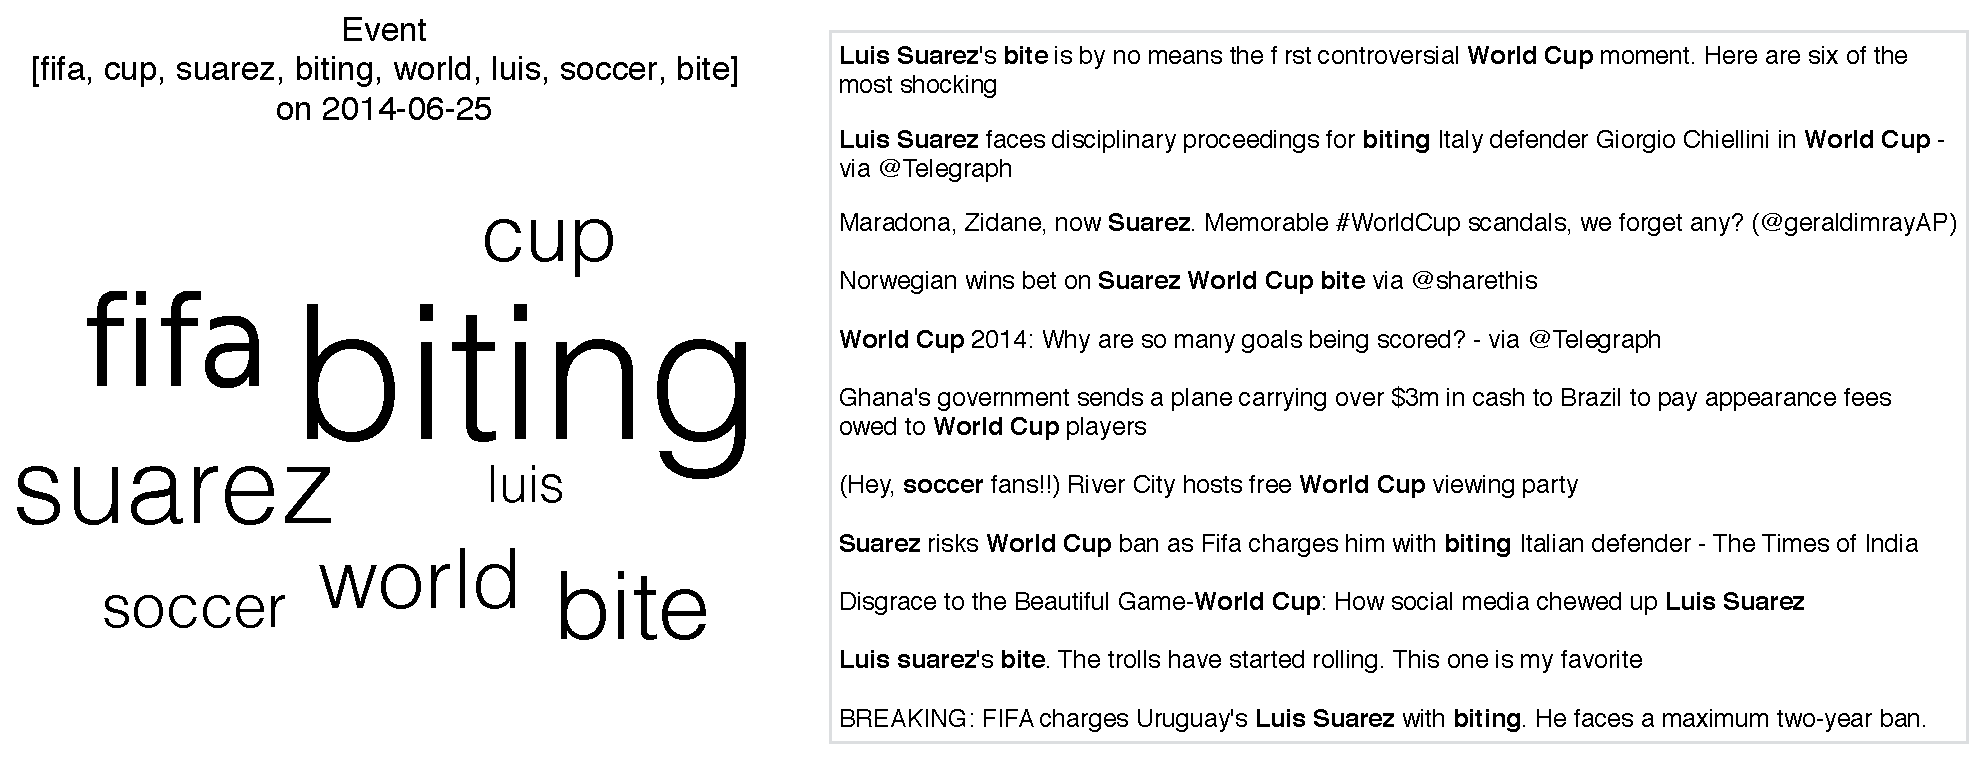
\includegraphics[width=\textwidth]{PLOSONE/figures/plots_revision/fig2}
  \caption[Example event collected using methodology]{{An example event, collected on 06/25/2014
      with keywords (left) and sample user posts (right) obtained
      from the Twitter Search API. The tweets in the event contain at
      least a pair of descriptive keywords and were retrieved close to the time
      of the event.}}
  \label{fig:fig2}
\end{figure}

The collection of events is converted into their VQ-event model
representation. Using this model, we can identify events that have
produced similar levels of activity in the social network. In other
words, events are considered to have similar activity if the
interarrival times between their social media posts are similarly
distributed, implying a very much alike collective reaction from users
to the events within a group. In order to identify groups of similar
events, we cluster the event models. We sort the resulting groups of
events from highest to lowest activity, according to the concentration
of social media posts in the bins that correspond to short
interarrival times. We consider the events that fall in the top
cluster to be high-activity events as most of their interarrival times
are concentrated in the smallest interval of the VQ-event model.  In
our dataset, these correspond to roughly 8\% of the events.  We
consider the next clusters in the sorted ranking to form medium-high
activity events, and so on.  Thus we end with four groups of events:
high, medium-high, medium-low and low. Fig~\ref{fig:fig3} shows a
heatmap of the interarrival relative frequency for each cluster. This
classification of events based on activity intensity is independent of
event size. More details of this methodology are provided in S1 Appendix.

\begin{figure}[!htb]
    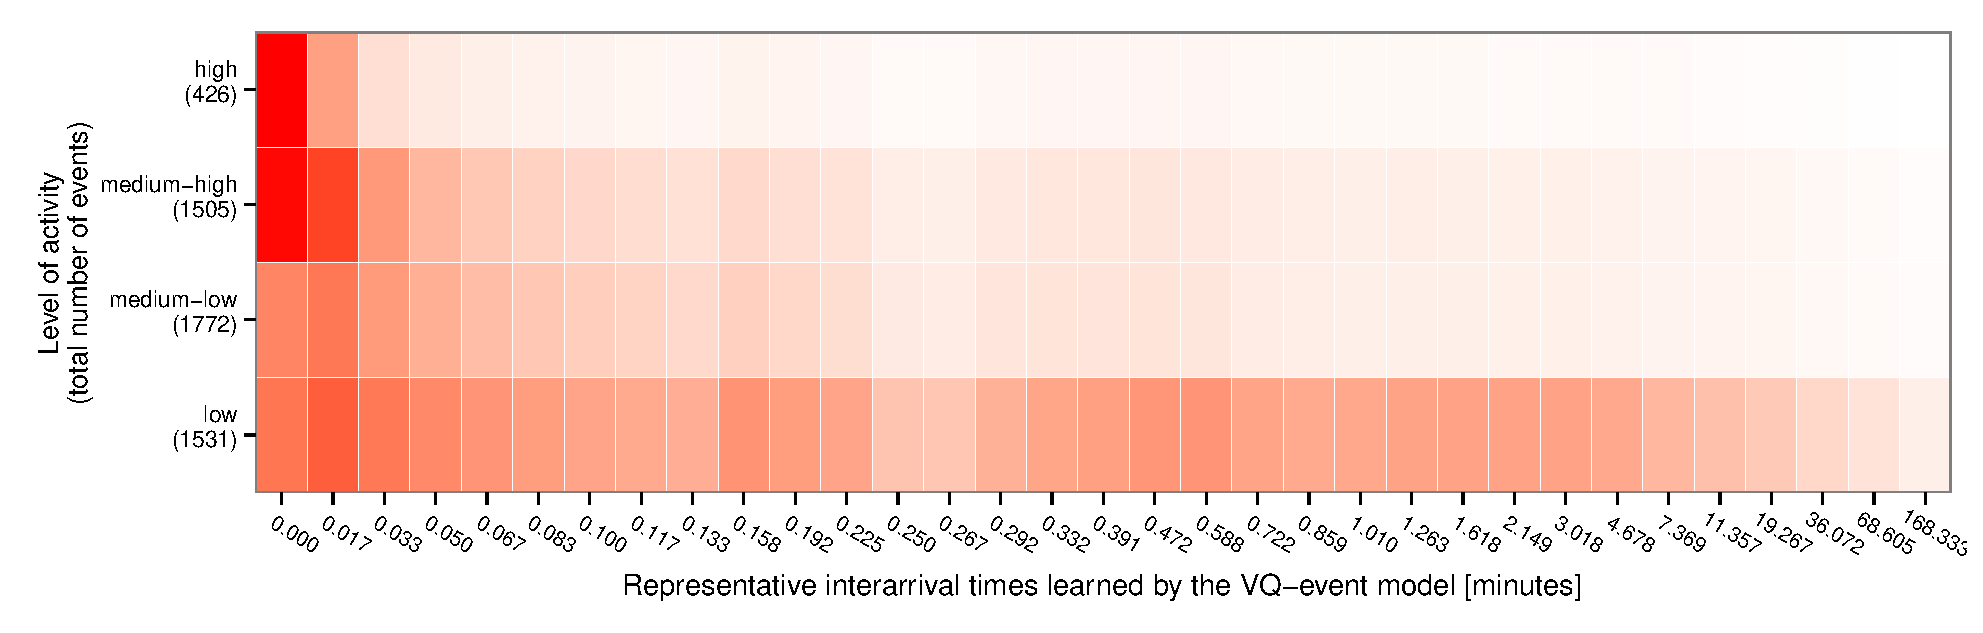
\includegraphics[width=\textwidth]{PLOSONE/figures/plots_revision/fig3}
  \caption[Event representation]{{Each row is the average representation of all the
      events in a cluster.  A darker cell represents a higher
      relative frequency value.  The y-axis specifies the number of events in
      each
      cluster.  Clusters are (top to bottom): high-activity, medium-high
      medium-low and low.}
    % \inote{Mauricio: change labels of x and y-axis (to: Event type
    % (total number of events))}
  }
  \label{fig:fig3}
\end{figure}

% Results and Discussion can be combined.
\section{Results and Discussion}
%\newtext{ 
Our main objective in this work is to analyze the
  characteristics of high-activity events which differentiate them from
  other types of events. In particular, we identify how early on in an
  event's lifecycle can we determine if an event is going
  produce high activity in the on-line social network.

Tables~\ref{table:high-impact-sample}
and~\ref{table:low-impact-sample} show examples of events from the
high-activity category and low-activity category. We recall that the
high-activity events are those which were in the top 8\% of the
ranking obtained by sorting the event clusters according to
concentration of interarrival times of social media posts in the
shortest interarrival time of the VQ-event model.  Table
\ref{table:high-impact-sample} shows two events of different sizes
(large and small) and different scopes (one global and the other of
more local scope) categorized as high activity in our dataset. The
first event, the death of Nelson Mandela, is one of the largest events
in the dataset, with $\approx 134,000$ tweets. The histogram
representation of this event, shown in Fig~\ref{fig:fig1}, suggests
that more than $80\%$ of the activity of the event was produced in
high-activity periods.  This is an event of international, political,
and social importance, that produced an overwhelming flood of messages
on social media. %% add detail about reach and scope 
Hence, it makes
sense for such an example to be a high-activity event.  The second
event, on the other hand, about the 2013 Mumbai Gang Rape is of much
smaller scale, with a total of $\approx 1,700$ tweets.  However, this
event caused considerable amount of immediate reaction on social
media, with close to $50\%$ of its activity concentrated within
high-activity periods. Despite its smaller size, in comparison to the
previous event, this event displays a similar reaction to that of
other high-activity events, but at a smaller scale. 
%More detailed
%inspection of the event shows that geolocated users which discussed
%this event were mostly from India and the U.K. In addition, we find
%that in the following days other events that are repercussions of this
%event gather a great deal of attention (with $\approx 12,700$
%tweets). % is it good to include this fact??

Table \ref{table:low-impact-sample} shows events that have been
classified by our methodology in the category of low activity.  The
first event, about a teen surviving after hiding in the wheel of a
airplane, had only a little more than $25\%$ of its messages arriving
with high-activity bursts although it had over $18,000$ messages.  The
second event, about the damages caused by a tornado in Canada, did not
garner much immediacy in attention of Twitter users, with only $7\%$
of its messages produced with short interarrival times. Most of the
messages of this event were well spaced out in time. Even though we
cannot say whether or not this event had significant implications in
the real-world, we can say that it did not have considerable impact on
the Twitter network. The lack of interest could be due to several
factors that are currently beyond the scope of this work, ranging from
the lack of Twitter users in the locality of the real-world event, to
it not being considered urgent by Twitter users. We intend to research
the relation between the real-world impact of an event and the network
reaction in future work.


%%%%%%%%% REWRITE ANALYSIS OF HISTOGRAM DISTRIBUTIONS %%%%%%%%%%%%

% Fig.~\ref{fig:highest}, Fig.~\ref{fig:low}, Fig.~\ref{fig:cdf-highest} and
% Fig.~\ref{fig:cdf-lowest} show the average histograms and the average
% cumulative distribution functions of the events corresponding to the
% high and low activity categories, respectively.  Visually, the average
% high-activity event vector representations starkly differ from that of
% a low-activity event in that the histogram in Fig.~\ref{fig:highest}
% seems to possess an exponential decay, while the histogram in
% Fig.~\ref{fig:low} does not.  To test this hypothesis, we fit
% exponential function of the form $f(x)=ae^{bx}$ to the event
% histograms. Table~\ref{tab:curve_fitting} summarizes the results from
% statistical significance tests performed on the parameters $a$ and
% $b$, and on the residual least squares error used for fitting the
% exponential curves.  The differences between these values is
% statistically significant ($p$-value $\leq2.2\times 10^{-16}$), thus demonstrating
% that high-activity events, on an average, fit the exponential decay
% curve much better than their low-activity counterparts.  In addition,
% Fig.~\ref{fig:param_est} shows two scatter plots with the resulting
% exponential parameters $a$ and $b$.  We observe that the majority
% ($97.4\%$) of high-activity events have an exponent $b \leq -50$,
% separating them unequivocally from other events.

%}


Fig~\ref{fig:fig4} shows the average histograms for events that
belong to the high activity, medium-high activity, medium-low activity
and low-activity clusters (displayed from left to right and top to
bottom). All histograms show a quick decay in average relative
frequency (resembling a distribution from the exponential family). In
particular, the high-activity group concentrates most of its activity
in the shortest interarrival rate, with lower activity groups mostly
concentrating their activity in the second bin with slower
decay. Fig~\ref{fig:fig5} further characterizes the differences in
behavior of the high and low-activity groups, showing that
high-activity events concentrate on average $70\%$ fo their activity
in the smallest bin ($0$ sec.), against $8\%$ for low-activity
events. In addition, Fig~\ref{fig:fig6} (left) shows the cumulative
distribution function (CDF) for each group of events, and
Fig~\ref{fig:fig6} (right) shows $\log{(1 - \mathrm{CDF})}$. Visual
inspection shows a clear difference in how interarrival rates are
distributed within each group, however, these figures do not indicate a
power-law distribution nor exponential distribution.%%

%%% Table with example tweets for events
\begin{table}[!htb]
  \centering
  {\scriptsize
    \begin{tabular*}{1\linewidth}{p{5cm}p{5cm}}
      \toprule
      \textbf{Event} & \textbf{Sample Tweets} \\
      \midrule
      \pbox{20cm}{\textbf{Description:}\\ Death of South African\\ politician Nelson Mandela. \vspace{.1cm}\\
        \textbf{Keywords:}\\ {[}nelson, mandela{]}\vspace{.1cm}\\
        \textbf{Date:}\\ 2013-12-05 \vspace{.1cm}\\
        \textbf{Size:} \\ 134,637 tweets}
      & \pbox{20cm}{
        @DaniellePeazer: RIP Nelson Mandela..... what a truly phenomenal and\\ inspirational man xx\vspace{.1cm}\\
        @iansomerhalder: Im in tears.The world has lost one of its greatest shepherds \\of peace. Thank you Mr.Mandela for the love you radiated. http://t.co/u39MVVEKe8\vspace{.1cm}\\
        @FootballFunnys: This is so true. RIP Nelson Mandela. http://t.co/vF9xri8LdP\vspace{.1cm}\\
        @David\_Cameron: I've spoken to the Speaker and there will be statements \\and tributes to Nelson Mandela in the House on Monday.} \\
      \midrule
      \pbox{20cm}{\textbf{Description:}\\ 2013 Mumbai Gang Rape \vspace{.1cm}\\
        \textbf{Keywords:}\\ {[}rape, mumbai{]}\vspace{.1cm}\\
        \textbf{Date:}\\ 2013-08-24 \vspace{.1cm}\\
        \textbf{Size:} \\1,705 tweets}
      & \pbox{20cm}{
      % select user.screen_name, text from tweet join user on tweet.user_id_id = user.user_id where event_id_id = 272;
      @TheNewsRoundup: Mumbai gang-rape: Second accused confesses to crime: \\Mumbai Police - Daily News Analysis http://t.co/KnabwhqH66\vspace{.1cm}\\
      @vijayarumugam: An interesting take on the Mumbai rape: http://t.co/ylBmW4l8sA\vspace{.1cm}\\
      @LondonStephanie: Two arrested over gang rape of Mumbai photojournalist \\that sparked renewed protests in India http://t.co/McYfLNDvaE\vspace{.1cm}\\
      @GanapathyI: Most brutal rapist of Delhi gang-rape was 17. Most brutal rapist\\ of Mumbai gang-rape is 18. Worst Young generation I have seen in my life.}\\
%        @M\_arioBalotelli: CLEAR ANGLE of the Suarez bite!!  https://t.co/bI08YsZWSE\vspace{.1cm}\\
%        @fifamedia: Disciplinary proceedings opened against Uruguay's Luis Suarez\\ http://t.co/w6mRNuSGZt\vspace{.1cm}\\
%        @DeadlineDayLive: Luis Suarez will sign a 5-year contract at Barcelona and he'll wear \\the no. 9 shirt. (Source: http://t.co/6uRIUwjsGN) http://t.co/FxyOf9ERVr\vspace{.1cm}\\
%        @GeniusFootball: BREAKING: FIFA have caught Suarez leaving the stadium?\\ http://t.co/vsQQCVV1GQ} \\
      \bottomrule
    \end{tabular*}
  }
  \caption[High-activity events examples]{{
        Examples of high-activity news events. The events
      shown were taken from the ``high'' category according to
Fig.~\ref{fig:fig4}.
        }}
  \label{table:high-impact-sample}
\end{table}

\begin{table}[!htb]
  \centering
  {\scriptsize
    \begin{tabular*}{1\linewidth}{p{5cm}p{5cm}}
      \toprule
      \textbf{Event} & \textbf{Sample Tweets} \\
      \midrule
      \pbox{20cm}{\textbf{Description:}\\Teen survives hiding \\in a plane wheel.\vspace{.1cm}\\
        \textbf{Keywords:}\\ {[}teen, survives, old, \\well, skydivers, plane, wheel, flight{]}\vspace{.1cm}\\
        \textbf{Date:}\\ 2014-04-21 \vspace{.1cm}\\
        \textbf{Size:}\\ 18,519}
      & \pbox{20cm}{
        %select user.screen_name, text from tweet join user on tweet.user_id_id = user.user_id where event_id_id in (22310,22274,22240);
        @ToniWoemmel: 16-year-old somehow survives flight from California to\\ Hawaii stowed away in planes wheel well: http://t.co/IGiJa60SiK\vspace{.1cm}\\
        @iOver\_think: 38,000 feet at -80F: Teen stowaway survives five-hour\\ California-to-Hawaii flight in wheel well http://t.co/ejXQH9VZyT\vspace{.1cm}\\
        @TruEntModels: GOD IS GOOD...runaway TEEN hid in plane's wheel for\\ 5 HOUR flight during FREEZING temps and survived http://t.co/6g6Cqhs9Ib\vspace{.1cm}\\
        @DvdVill: A 16-year-old kid, who was mad at his parents, hid inside a jet\\ wheel and survived flight to Hawaii. http://t.co/c82GbjrfUH\\
        %@guardiannews: Angela Merkel denied access to her NSA file http://t.co/FLQc0zSjYJ\vspace{.1cm}\\
        %@mog7546: \#GERMANY's \#Merkel says \#OBAMA's \#US assurances on \#NSA spying\\ "INSUFFICIENT" - Reuters India http://t.co/D2L52CP9YZ\vspace{.1cm}\\
        %@GermanyForum: Merkel denied access to own NSA file http://t.co/e6vKCOkbXA\vspace{.1cm}\\
        %@kgosztola: US ignores request from German Chancellor Angela \\Merkel to look at NSA file:\\ http://t.co/HFTMMZBu5W
      }
      \\
            \midrule
      \pbox{20cm}{\textbf{Description:}\\Surveying the damages of \\ recent tornado in Canada. \vspace{.1cm}\\
        \textbf{Keywords:}\\ {[}canada, tornado{]}\vspace{.1cm}\\
        \textbf{Date:}\\ 2014-06-21 \vspace{.1cm}\\
        \textbf{Size:}\\ 1,033}
      & \pbox{20cm}{
        @Kathleen\_Wynne: Visited \#Angus today to survey the damage. Thankfully no \\fatalities or major injuries from recent tornado. http://t.co/xRQyRWg5Vw\vspace{.1cm}\\
        @SunNewsNetwork: PHOTOS \& VIDEO: Hundreds displaced after \\ tornado hits Ontario town, destroying homes http://t.co/L38rG6N1a6\vspace{.1cm}\\
        @CBCToronto: Kathleen Wynne is speaking at site of tornado damage in Angus, \\Ont. now. Watch live here: http://t.co/EDKNUiZo0X \#cbcto\vspace{.1cm}\\
        @InsuranceBureau: @CTVBarrieNews: Insurance Bureau of Canada is setting up \\a mobile unit in \#Angus today to help residents affected by \#Tornado}
      \\
      \bottomrule
    \end{tabular*}
  }
  \caption[Low-activity events examples]{{
                Examples of events with low activity. The events
      shown were taken from the ``low'' category according to
Fig.~\ref{fig:fig4}}
          .}
  \label{table:low-impact-sample}
\end{table}

%%\clearpage
\begin{table}
  \centering
  {\scriptsize
    \begin{tabular*}{1\linewidth}{p{5cm}p{5cm}}
      \toprule
      \textbf{Event} & \textbf{Sample Tweets} \\
      \midrule
      \pbox{20cm}{\textbf{Description:}\\ Death of South African\\ politician Nelson Mandela. \vspace{.1cm}\\
        \textbf{Keywords:}\\ {[}nelson, mandela{]}\vspace{.1cm}\\
        \textbf{Date:}\\ 2013-12-05 \vspace{.1cm}\\
        \textbf{Size:} \\ 134,637 tweets}
      & \pbox{20cm}{
        @DaniellePeazer: RIP Nelson Mandela..... what a truly phenomenal and\\ inspirational man xx\vspace{.1cm}\\
        @iansomerhalder: Im in tears.The world has lost one of its greatest shepherds \\of peace. Thank you Mr.Mandela for the love you radiated. http://t.co/u39MVVEKe8\vspace{.1cm}\\
        @FootballFunnys: This is so true. RIP Nelson Mandela. http://t.co/vF9xri8LdP\vspace{.1cm}\\
        @David\_Cameron: I've spoken to the Speaker and there will be statements \\and tributes to Nelson Mandela in the House on Monday.} \\
      \midrule
      \pbox{20cm}{\textbf{Description:}\\ 2013 Mumbai Gang Rape \vspace{.1cm}\\
        \textbf{Keywords:}\\ {[}rape, mumbai{]}\vspace{.1cm}\\
        \textbf{Date:}\\ 2013-08-24 \vspace{.1cm}\\
        \textbf{Size:} \\1,705 tweets}
      & \pbox{20cm}{
      % select user.screen_name, text from tweet join user on tweet.user_id_id = user.user_id where event_id_id = 272;
      @TheNewsRoundup: Mumbai gang-rape: Second accused confesses to crime: \\Mumbai Police - Daily News Analysis http://t.co/KnabwhqH66\vspace{.1cm}\\
      @vijayarumugam: An interesting take on the Mumbai rape: http://t.co/ylBmW4l8sA\vspace{.1cm}\\
      @LondonStephanie: Two arrested over gang rape of Mumbai photojournalist \\that sparked renewed protests in India http://t.co/McYfLNDvaE\vspace{.1cm}\\
      @GanapathyI: Most brutal rapist of Delhi gang-rape was 17. Most brutal rapist\\ of Mumbai gang-rape is 18. Worst Young generation I have seen in my life.}\\
%        @M\_arioBalotelli: CLEAR ANGLE of the Suarez bite!!  https://t.co/bI08YsZWSE\vspace{.1cm}\\
%        @fifamedia: Disciplinary proceedings opened against Uruguay's Luis Suarez\\ http://t.co/w6mRNuSGZt\vspace{.1cm}\\
%        @DeadlineDayLive: Luis Suarez will sign a 5-year contract at Barcelona and he'll wear \\the no. 9 shirt. (Source: http://t.co/6uRIUwjsGN) http://t.co/FxyOf9ERVr\vspace{.1cm}\\
%        @GeniusFootball: BREAKING: FIFA have caught Suarez leaving the stadium?\\ http://t.co/vsQQCVV1GQ} \\
      \bottomrule
    \end{tabular*}
  }
  \caption{\textbf{\textcolor{blue}{
        Examples of high-impact news events. The events
      shown were taken from the ``high'' category according to Fig.~\ref{fig:low_buzz_high_buzz}.}.
        }}
  \label{table:high-impact-sample}
\end{table}

\begin{table}
  \centering
  {\scriptsize
    \begin{tabular*}{1\linewidth}{p{5cm}p{5cm}}
      \toprule
      \textbf{Event} & \textbf{Sample Tweets} \\
      \midrule
      \pbox{20cm}{\textbf{Description:}\\Teen survives hiding \\in a plane wheel.\vspace{.1cm}\\
        \textbf{Keywords:}\\ {[}teen, survives, old, \\well, skydivers, plane, wheel, flight{]}\vspace{.1cm}\\
        \textbf{Date:}\\ 2014-04-21 \vspace{.1cm}\\
        \textbf{Size:}\\ 18,519}
      & \pbox{20cm}{
        %select user.screen_name, text from tweet join user on tweet.user_id_id = user.user_id where event_id_id in (22310,22274,22240);
        @ToniWoemmel: 16-year-old somehow survives flight from California to\\ Hawaii stowed away in planes wheel well: http://t.co/IGiJa60SiK\vspace{.1cm}\\
        @iOver\_think: 38,000 feet at -80F: Teen stowaway survives five-hour\\ California-to-Hawaii flight in wheel well http://t.co/ejXQH9VZyT\vspace{.1cm}\\
        @TruEntModels: GOD IS GOOD...runaway TEEN hid in plane's wheel for\\ 5 HOUR flight during FREEZING temps and survived http://t.co/6g6Cqhs9Ib\vspace{.1cm}\\
        @DvdVill: A 16-year-old kid, who was mad at his parents, hid inside a jet\\ wheel and survived flight to Hawaii. http://t.co/c82GbjrfUH\\
        %@guardiannews: Angela Merkel denied access to her NSA file http://t.co/FLQc0zSjYJ\vspace{.1cm}\\
        %@mog7546: \#GERMANY's \#Merkel says \#OBAMA's \#US assurances on \#NSA spying\\ "INSUFFICIENT" - Reuters India http://t.co/D2L52CP9YZ\vspace{.1cm}\\
        %@GermanyForum: Merkel denied access to own NSA file http://t.co/e6vKCOkbXA\vspace{.1cm}\\
        %@kgosztola: US ignores request from German Chancellor Angela \\Merkel to look at NSA file:\\ http://t.co/HFTMMZBu5W
      }
      \\
            \midrule
      \pbox{20cm}{\textbf{Description:}\\Surveying the damages of \\ recent tornado in Canada. \vspace{.1cm}\\
        \textbf{Keywords:}\\ {[}canada, tornado{]}\vspace{.1cm}\\
        \textbf{Date:}\\ 2014-06-21 \vspace{.1cm}\\
        \textbf{Size:}\\ 1,033}
      & \pbox{20cm}{
        @Kathleen\_Wynne: Visited \#Angus today to survey the damage. Thankfully no \\fatalities or major injuries from recent tornado. http://t.co/xRQyRWg5Vw\vspace{.1cm}\\
        @SunNewsNetwork: PHOTOS \& VIDEO: Hundreds displaced after \\ tornado hits Ontario town, destroying homes http://t.co/L38rG6N1a6\vspace{.1cm}\\
        @CBCToronto: Kathleen Wynne is speaking at site of tornado damage in Angus, \\Ont. now. Watch live here: http://t.co/EDKNUiZo0X \#cbcto\vspace{.1cm}\\
        @InsuranceBureau: @CTVBarrieNews: Insurance Bureau of Canada is setting up \\a mobile unit in \#Angus today to help residents affected by \#Tornado}
      \\
      \bottomrule
    \end{tabular*}
  }
  \caption{\textbf{\textcolor{blue}{
                Examples of events with low impact. The events
      shown were taken from the ``low'' category according to Fig.~\ref{fig:low_buzz_high_buzz}}
                }.}
  \label{table:low-impact-sample}
\end{table}


\begin{figure}[!htb]
  \centering
    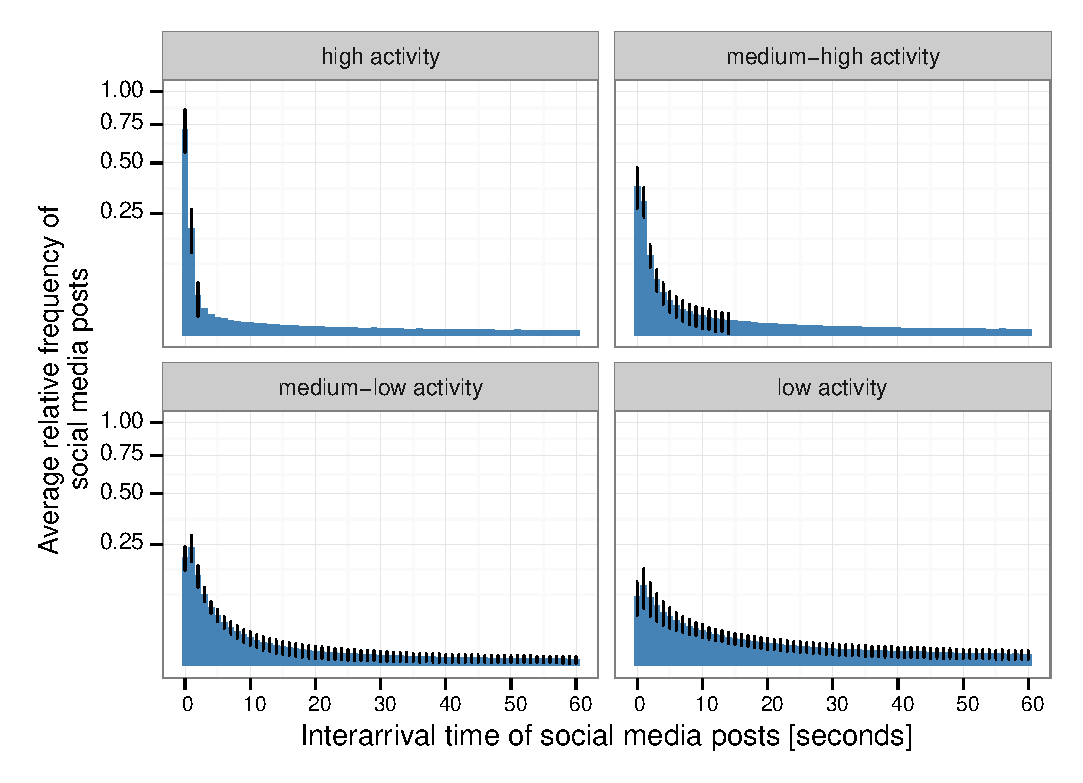
\includegraphics[width=\textwidth]{PLOSONE/figures/plots_revision/fig4}
  \caption[Average histograms of events from different categories.]{{Average histograms of the high activity,
      medium-high activity, medium-low activity and low activity
      clusters in our dataset (from left to right and top to
      bottom). All histograms include standard deviation bars and were
      cut-off at 60 second length for better visibility.
      % \inote{change labels of x and y axis}
    }}\label{fig:fig4}
\end{figure}

\begin{figure}[!htb]
  \centering
    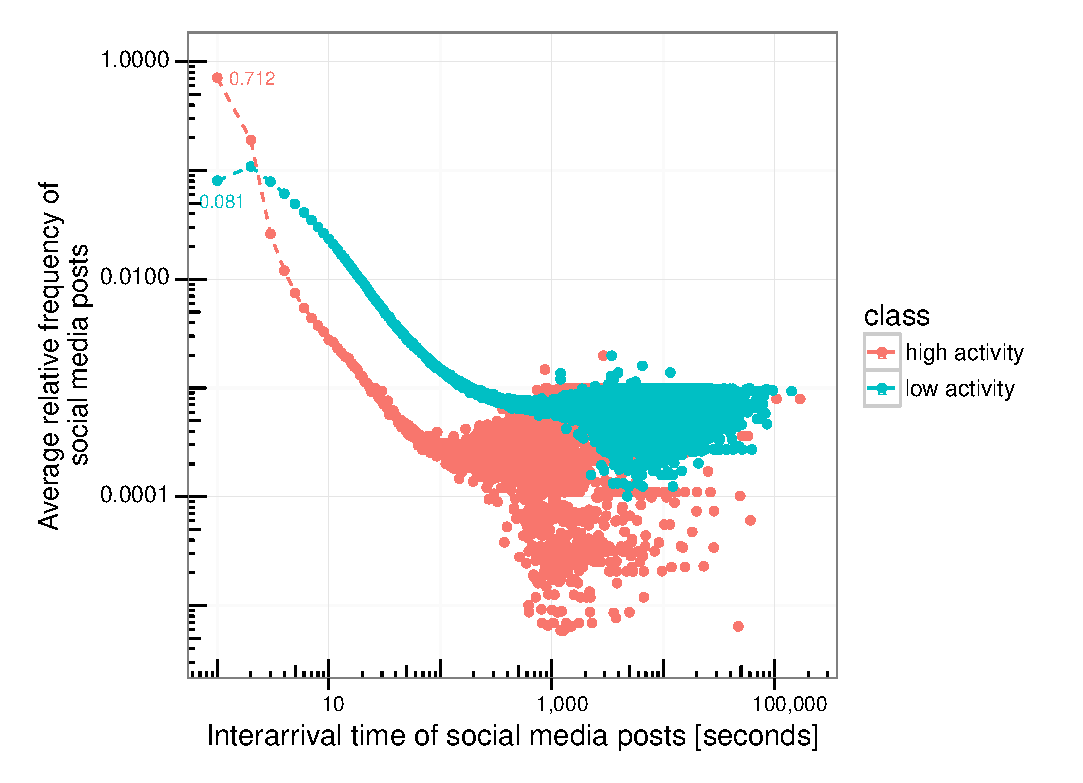
\includegraphics[width=\textwidth]{PLOSONE/figures/plots_revision/fig5}
  \caption[Scatter plots of interarrival times]{{Scatter plots of the average relative frequencies of interarrival times
for the high-activity and low-activity clusters of events (i.e., scatter
plots of the histograms in Fig~\ref{fig:fig4} in log-log scale). $y$-axis
represents the average relative frequency of social media messages and
$x$-axis the interarrival time.
    }}\label{fig:fig5}
\end{figure}

\begin{figure}[!htb]
  \centering
 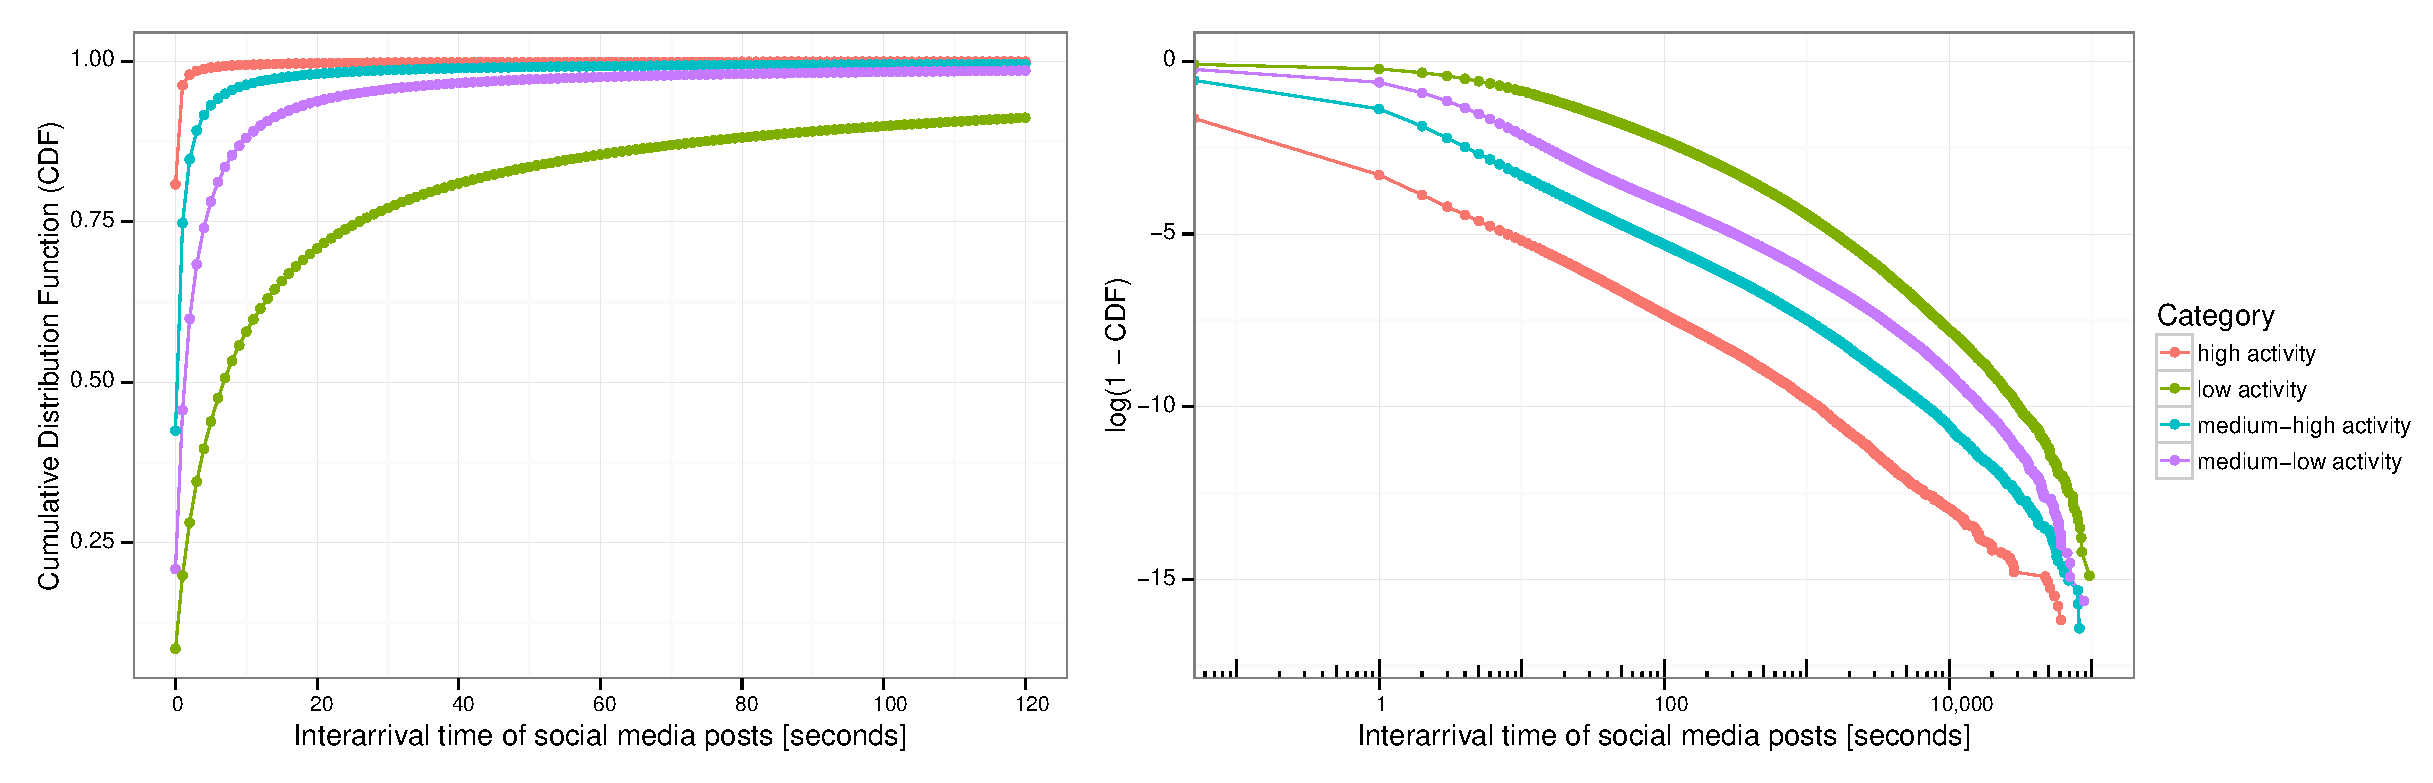
\includegraphics[width=\textwidth]{PLOSONE/figures/plots_revision/fig6_log}
  \caption[CDF for events from different categories]{{(Left) Average cumulative distribution function (CDF) for
the high activity, medium-high activity, medium-low activity and low activity clusters in our dataset.
(Right) $\log{(1 - \mathrm{CDF})}$ for the same clusters. 
      % \inote{change labels of x and y axis}
    }}\label{fig:fig6} %% fig6_long_inf_omitted.pdf
\end{figure}

Further analysis of the high-activity events shows significant
differences to other events, in the following aspects: (i) how the
information about these events is propagated, (ii) the characteristics
of the conversations that they generate, and (iii) how focused users
are on the news topic. In detail, high-activity events have a higher
fraction of {\em retweets} (or shares) relative to their overall
message volume. On average, a tweet from a high-activity event is
retweeted 2.36 times more than a tweet from a low activity event. The
most retweeted message in high-activity events is retweeted 7 times more
than the most retweeted message in a medium or low activity event. We
find that a small set of initial social media posts are propagated
quickly and extensively through the network without any rephrasing by
the user (just plain forwarding). Intuitively, this seems justified given
general topic urgency of high-activity events. Events that are not
high-activity did not exhibit these characteristics.

Our research also revealed that high-activity events tend to spark more conversation
between users, 33.4\% more than other events. This is reflected in the
number of {\em replies} to social media posts. The number of different
users that engage with high-activity events is 32.7\% higher than in
events that are not high-activity. Posts about high-activity events are
much more topic focused than in other events. The vocabulary of unique
words as well as {\em hashtags} used in high-activity events is much
more narrow than for other events. Medium and low activity events have
over 7 times more unique hashtags than high-activity events. This is
intuitive, given that if a news item is sensational, people will
seldom deviate from the main conversation topic.

% We have presented an analysis of high-impact news events based on
% the data of their entire life-cycle in the social network. We used
% the arrival time intervals to create a model that allows us to
% classify the event according to its impact. Nevertheless,

In a real-world scenario, in order to predict if an early breaking
news story will have a considerable impact in the social network, we
will not have enough data to create its activity-based model, i.e., we
will not yet know the distribution of the speed at which the social
media posts will arrive for the event. For instance, an event can
start slowly and later produce an explosive reaction, or start
explosively and decay quickly to an overall slower message arrival
rate. Still, reliable early prediction of very high-activity news is
important in many aspects, from decisions of mass media information
coverage, to natural disaster management, brand and political image
monitoring, and so on.

For the task of early prediction of high-activity events we use features 
that are independent of our activity-based model such as
the retweets, the sentiment of the posts about the event, etc. 
These features are computed on the early 5\% of messages about the event.
% More details are provided in the supplementary material.
The results are an average from a 5-fold cross validation with
randomly selected 60\% training, 20\% validation and 20\% test splits.
The high-activity events are identified with a precision of 82\% using
only the earliest 5\% of the data of each event
(Table~\ref{tab:classification_results}).  Additionally, we were able to
identify with high accuracy a considerable percentage of all
high-activity events ($\approx 46\%$) at an early stage, with very few
false positives (Table~\ref{tab:classification_results} and~\ref{tab:confusion_matrix}).

\begin{table}[!htb]
  %\begin{adjustwidth}{-10mm}{-10mm}
  \centering
  {\scriptsize
    \begin{tabularx}{\textwidth}{lcccc|cccc}
      \toprule
      & \multicolumn{4}{c}{\textbf{Early 5\% Tweets}} & \multicolumn{4}{c}{\textbf{All Tweets}} \\
      \midrule
      & FP-Rate & Precision & Recall & ROC-area & FP-Rate & Precision & Recall & ROC-area \\
      % \midrule
      high & 0.009 & 0.819 & 0.455 & 0.900 & 0.01 & 0.830 & 0.540 & 0.945 \\
      non-high & 0.545 & 0.954 & 0.991 & 0.900 &  0.460 & 0.960 & 0.990 & 0.945 \\
      \bottomrule
    \end{tabularx}
  }
  \caption[Classification of high-activity events]{{Classification of high-activity events.}}
  \label{tab:classification_results}
  %\end{adjustwidth}
%                                                                                                                                448,1         93%
\end{table}

\begin{table}[!htb]
  \centering
  % {\scriptsize
  \begin{tabularx}{\textwidth}{lcc|cc}
    \toprule
    \multirow{2}{*}{ }& \multicolumn{2}{c}{\textbf{Early 5\% Tweets}} & \multicolumn{2}{c}{\textbf{All Tweets}} \\
    \midrule
    % \cmidrule{2-5} \cline{2-5}
    & high-activity & non-high-activity & high-activity & non-high-activity \\
    % \midrule
    high-activity & $194$ & $232$ & $230$ & $196$\\
    non-high-activity & $43$ & 4,765 & 47 & 4,761 \\
    \bottomrule
  \end{tabularx}
  % }
  \caption[Confusion matrix for high-activity event prediction]{{Confusion matrix for high-activity events prediction.}}
  \label{tab:confusion_matrix}
\end{table}



The precision using only the early tweets is almost as good as using
all tweets in the event (0.819 to 0.830). This suggests that the
social network somehow acts as a natural filter in separating out the
high-activity events fairly early on.  The recall goes from 0.455 to
0.540. This indicates that there are some high-activity events which
require more data in order to determine what kind of activity they will
produce, or events for which activity occurs due to random conditions. A
detailed description of the features and different classification
settings are provided in the supplementary material.%\supplementary.




\section{Conclusion}

We study the characteristics of the activity that real-world news produces
in the Twitter social network. In particular, we propose to measure the impact of the
real-world news event on the on-line social network by modeling the user
activity related to the event using the distribution of their
interarrival times between consecutive messages. In our research we observe
that the activity triggered by real-world news events follows a similar
pattern to that observed in other types of collective reactions to events.
This is, by displaying periods of intense activity as well as long periods of
inactivity. We further extend this analysis by identifying groups of events
that produce much more concentration of high-activity than other events. 
We show that there are several specific properties that distinguish how
high-activity events evolve in Twitter, when comparing them to other
events. We design a model for events, based on the codebook approach, that allows us to do
unambiguous classification of high-activity events based on the impact
displayed by social network. % This definition does not have some of the
%problems that current notions of virality and popularity have. 
Some notable
characteristics of high-activity events are that they are forwarded more
often by users, and generate a greater amount of conversation than
other events.  Social media posts from high-activity news events are
much more focused on the news topic. Our experiments show that there
are several properties that can suggest early on if an event will have
high-activity on the on-line community.  We can predict a high number of
high-activity events {\em before} the network has shown any type of
explosive reaction to them. % Using simple off-the-shelf feature based
%classifiers, we can
% predict many high-impact events with high precision.
This suggests that users are collectively quick at deciding whether an
event should receive priority or not.  However, there does exist a fraction of
events which will create high activity, despite not presenting
patterns of other high activity events during their early stages.  These
events are likely to be affected by other factors, such as random
conditions found in the social network at the moment and require
further investigation.

\chapter{Discovering Trends of Drug Abuse from Social Media Data}
\label{AB_chapter}
\section{Introduction}
Nonmedical use of prescription medications/drugs (NMUPD), 
particularly prescription analgesic opioid abuse, 
is a grave threat to the nation's health. 
In fact, the U.S. Centers for Disease Control and Prevention 
recorded a record number of drug overdose deaths in 2014, 
headlined by a nearly fourfold increase in prescription 
opioid-related drug mortality since 1999, 
further coupled by increased heroin injection drug use 
associated with NMUPD behavior 
(Centers for Disease Control and Prevention (CDC), 2011;  
Centers for Disease Control and Prevention (CDC), 2013; 
\cite{compton2016relationship}, \cite{rudd2016increases}). 
As this public health crisis continues to gain public attention, 
so does the need for better data identifying underlining 
NMUPD behaviors, trends, and risk factors in order to optimize 
efforts at improving access to treatment, 
preventing overdose, and ensuring community interventions are effective. 
Currently, existing NMUPD data is largely derived from national 
population-based surveys that measure the prevalence estimates, 
attitudes, and associated trends of various forms of substance abuse (including NMUPD) 
and rely upon respondents to self-report their past drug use 
behaviors via face-to-face interviews or self-administered questionnaires 
(\cite{katsuki2015establishing, schepis2016trends}). 
These survey-based instruments are critical in identifying 
generalizable trends of prescription drug abuse behavior in a 
national population, assessing changes in what classes of prescription drugs 
are becoming popular targets of abuse, and aid in the development of 
targeted interventions and policy to address risk and protective factors common to 
NMUPD \cite{han2015nonmedical}.

However, even powerful nationally representative surveys, 
such as the National Survey on Drug Use and Health and the Monitoring 
the Future survey (which focuses on students and young adults), 
have certain inherent limitations \cite{schepis2016trends,mccabe2012co,mccabe2013leftover}. 
Most evidently, they largely rely on respondents to self-report and recall recent 
and past drug abuse behavior, a methodology that can be subject to 
recall bias \cite{harrison1997validity}. Further, results from these 
surveys generally take time to compile after data collection is completed, 
with trends reported from these observations possibly changing by the time survey results are 
reported \cite{katsuki2015establishing}.

Hence, alternative methods for conducting surveillance of NMUPD 
behavior are needed to augment findings from national substance abuse 
surveys, including leveraging the power of ``big data" analysis and social media 
platforms that are now heavily populated by a wide demographic of the substance 
using population, a practice now popularized as ``digital epidemiology" or 
``infoveillance \cite{salathe2012digital}."

Despite, growing opportunities in a growing digitized social sphere, 
the massive size of these datasets and accompanying challenges of filtering, 
processing and analyzing the data in a meaningful way, has left the field ripe for 
innovation and improvement, particularly through cross-disciplinary research 
collaborations. In response, this study advances prior studies that have examined 
the linkages between Twitter and NMUPD and introduces a new methodology 
leveraging recent developments in computer science in order to gain a 
“bigger” picture of national NMUPD trends. Previous studies have used 
methodologies focusing on content analysis and human coding/annotation 
using keyword searches, identifying subsets of Twitter NMUPD-related 
social circles, and analyzing a random sample of filtered tweets 
\cite{hanson2013tweaking,hanson2013exploration,katsuki2015establishing,shutler2015drug}.

In this study, we similarly conducted surveillance of the popular 
microblogging site Twitter (which now commands 310 million active users) 
filtered for content posted by users that specifically mentioned 
prescription analgesic opioid drugs. However, because of the massive amount 
of data required to be analyzed and given that content on Twitter is not 
curated for information specifically relevant to NMUPD, Twitter datasets 
often contain a high number of tweets that are non-relevant to NMUPD 
(i.e. noise) compared to content that actually describes NMUPD-related 
behavior (i.e. signal content). This condition necessitates a methodology 
that can iteratively filter tweets to eliminate noise and only 
retain tweets relevant to NMUPD behavior similar to those used in 
other studies examining other important public health issues 
\cite{chen2014flu,prier2011identifying}. Concomitantly, by 
filtering only for NMUPD relevant content, this methodology 
subsequently analyzes the tweets to discover and identify the 
different underlying latent themes that exist in the entire dataset. 
Hence, our study's methodology differs from prior studies because 
it can be used to highly automate filtering and coding of an 
extremely large dataset of tweets and simultaneously 
identify key NMUPD themes that are occurring in the entire 
Twittersphere in order to better inform researchers and 
the public about changes in the prescription opioid epidemic.


\section{Methods}
\subsection{Overall aims}
This study was conducted in two distinct phases: 
data collection and data analysis. The goal of this study included 
two distinct aims related to data processing and analysis to identify 
risk behaviors associated with NMUPD as reported in content generated by Twitter users. 
The first aim was to increase the signal to noise ratio in 
the dataset of all tweets analyzed and weed out tweets that are not 
relevant to NMUPD behavior. The second involved identifying themes and
patterns from the large corpus of Tweets in order to gain a broader 
understanding of NMUPD behaviors for a larger Twitter user population that 
included more than 11 million tweets collected during a six-month period. 
In order to handle a dataset of this magnitude it is necessary to develop 
methodologies to be as automated as possible and limit the amount of human coding, 
in order to scale big data collection, surveillance and analysis. 
Section \ref{AB:data_collection} 
describes the data collection process used to generate large amounts of 
tweets on NMUPD from the Twitter Application Programming Interface (API) stream. 
Section \ref{AB:analysis_plan} describes the 
iterative methodology that was employed to 
increase the signal to noise ratio in the dataset, 
and to identify patterns and themes present in the data specific to analgesic opioid NMUPD.

\subsection{Data collection}
\label{AB:data_collection}
Twitter provides a public API that enables the collection 
of messages publicly posted by its users via its online platform. 
We used a data collection methodology involving cloud-based computing 
services offered by Amazon Web Services (AWS) and virtual computers via 
Amazon EC2 t2.micro instances set to filter and collect tweet 
objects containing specific NMUPD keywords.

Keywords included brand and international non-proprietary 
(e.g. generic) names (INN names) of commonly abused prescription 
analgesic opioid drugs. The data collection methodology used 
for this study has been previously described in detail in a prior 
published study (\cite{katsuki2015establishing}). 
INN names of prescription opioid drugs included: Percocet (acetaminophen/oxycodone),
OxyContin (oxycodone) and Oxycodone and were used in conjunction 
with the streaming API in order to track tweet objects that potentially 
contain at least one of these keywords. This generated a total of 
approximately 11M English-language tweets that were collected 
between the period of June and November 2015. A summary of the 
number of tweets collected for each drug is provided in Table \ref{table:drugs_summary}. 
Additionally, during the preprocessing of the data, 
any identifiable information (e.g. Twitter account names, etc.) 
was removed from prior to data analysis.

\begin{table}
\centering
\begin{tabular}{|c|c|c|}
\hline
Keywords &   \#-of-tweets & \% of English tweets \\
Percocet &  8,004,229  & 94.24 \\
OxyContin & 3,280,910  & 92.16 \\
Oxycodone  & 2,315,321 &  88.90 \\
\hline
\end{tabular}
\caption[Summary of the number of tweets collected.]{Summary of keywords used in 
conjunction with the Twitter 
Streaming API for data collection and the corresponding number of tweets collected.}
\label{table:drugs_summary}
\end{table}

\subsection{Analysis Plan}
\label{AB:analysis_plan}

In order to appropriately code, identify, and characterize large 
volumes of data collected from social media sites in the context 
of public health issues, the application of machine learning has 
become a critical strategy in digital surveillance. The need for 
the application of machine learning has been necessitated by the 
sheer enormity of the data used for analysis when generating data 
from public sources like the Twitter API. Machine learning, especially 
unsupervised machine learning models are efficient at automatically 
finding patterns in the data and summarizing the content of the 
text corpus. The algorithms are computationally efficient and results 
have the advantage of not being affected by potential human judgment bias.

In the machine learning literature, there exist models which, 
when given a text corpus, are able to identify the underlying latent 
patterns or themes or (more formally in the machine learning 
literature) topics present in the corpus. Such models are 
referred to as topic models owing to their ability to summarize 
the content of the corpus concisely in terms of a few distinct topics 
\cite{blei2003}. With the advent of Twitter and other microblogging 
sites as a potent source of textual data, a model called the 
Biterm Topic Model (BTM) was proposed specifically to detect 
themes and patterns in corpora of short-texts \cite{yan2013biterm}.

The methodology for our work is built by using 
BTM as the core for recognizing patterns in our corpus of tweets. 
BTM, when given a corpus of tweets as a parameter $k$ 
for the number of themes to be identified as inputs identifies $k$ 
underlying themes in the corpus. This is the learning phase of 
BTM. As the output of this phase, it produces a discrete 
probability distribution for all words for each theme. 
Ideally, this distribution would place large weights on 
the words that are most representative of that theme. 
Hence, a ranking of the top-10 words produced by 
BTM for each theme can be used as a summary 
representing all the themes present in the input corpus.

BTM also operates in what is called the inference phase. 
In this phase, BTM has the ability to decompose each tweet 
in terms of the themes identified in the learning phase. 
As the output of this phase, BTM produces a histogram for 
each tweet where each bin represents a theme discovered in 
the learning phase. The value in that bin represents how 
correlated the given tweet is to that particular theme. 
A tweet highly correlated to a particular theme will have, 
in its histogram representation, a large weight placed 
in the corresponding bin. The inference phase of BTM 
essentially enables us to retrieve the tweets most 
correlated to a particular theme.

First, the dataset was separated according to the keywords filtered in Table \ref{table:drugs_summary}. 
Once a subset of tweets corresponding to each drug was obtained, 
a two-step iterative process was employed. 
The first step involved detecting $k$ themes from the set of tweets 
corresponding to each drug using the learning phase of BTM. 
The second step involved manually identifying themes that produced false positive 
content; i.e., content irrelevant to NMUPD behavior and promotion. 
For this step, the top ranked words in each theme 
(produced in the first step) were analyzed in conjunction 
with the inclusion/exclusion rules laid out in Table \ref{table:inclusion_exclusion} 
to determine whether or not a theme was relevant to NMUPD behavior.

\begin{table}
\centering{c}
\begin{tabular}{|c|}
\hline
\pbox{20cm}{Contains INN or slang names identified by NIDA of a prescription drug subject to abuse.}\\
\pbox{20cm}{Mentions of other illicit drugs (e.g., heroin, cocaine, marijuana) and/or alcohol.}\\
\pbox{20cm}{Mentions of identified substance abuse risk behavior (e.g. overdose, injection, withdrawal).}\\
\pbox{20cm}{Contains adjectives related to prescription drug abuse behavior (e.g., popping).}\\
\hline
\end{tabular}
\caption[Inclusion exclusion rules for topics.]{Summary of rules applied to determine if a theme was relevant for inclusion in subsequent iterations.}
\label{table:inclusion_exclusion}
\end{table}

Prior studies that have utilized content analysis and human annotation 
in order to filter out tweets that are not explicitly related to 
individual NMUPD behavior (e.g. tweets containing news reports, 
automated feeds, tweets by commercial entities, illicit online sales, etc.) 
\cite{katsuki2015establishing,hanson2013tweaking,hanson2013exploration,shutler2015drug}
(Hanson et al., 2013a; Hanson et al., 2013b; Katsuki et al., 2015 ;  Shutler et al., 2015). 
We used a similar filtering scheme instead relying upon our machine 
learning BTM protocol to identify tweets that contained 
NMUPD-related behavior content of interest. Specifically, relevance to NMUPD behavior focused on 
four specific conditions: 
\begin{enumerate}
\item contained INN or ``street"/slang term for a prescription opioid drug subject to abuse; 
\item mentioned other prescription and/or illicit drug abuse (i.e. polydrug abuse); 
\item mentioned identified substance abuse risk behavior (e.g. overdose, injection, adverse event); and 
\item contained a commonly used adjective or verb related to NMUPD. 
\end{enumerate}

Once the themes satisfying conditions laid out in Table \ref{table:inclusion_exclusion} 
were identified, using the inference phase of BTM, the most 
correlated tweets to these themes were obtained and those not related were discarded.

These two steps were repeated in three iterative BTM rounds to improve 
content saturation and ensure that the filtered content was 
highly relevant to NMUPD behavior of interest. After each iteration, 
what remains is a smaller corpus of tweets with a higher signal to 
noise ratio than before. The number of themes to be discovered, i.e. the parameter $k$, 
needs to be set by the user. We set this number to $20$, $10$, and $7$ in the first, 
second and third round of iterations respectively in order to ensure 
appropriate thematic saturation balancing missing important 
emerging themes that could be detected. 
Figure \ref{fig:overview_methodology} summarizes our iterative data filtering methodology.

\begin{figure}
\centering
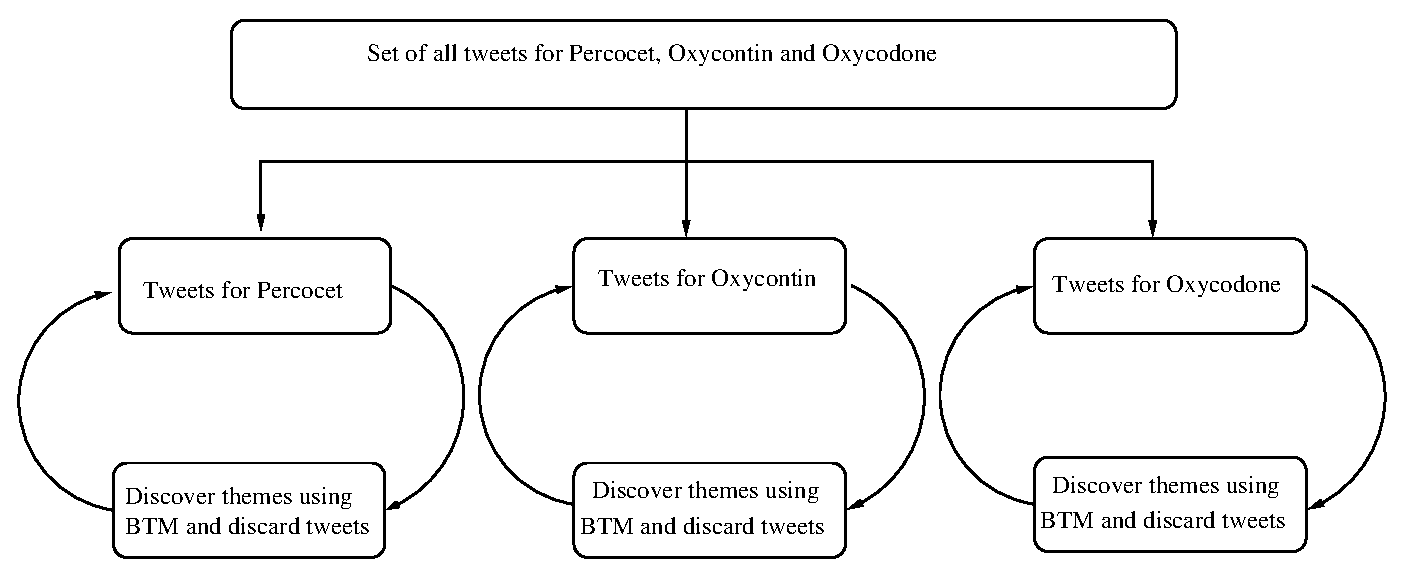
\includegraphics[width=\textwidth]{AB/chart}
\caption[Data analysis overview]{An overview of the steps undertaken in the interative BTM rounds applied to set of all tweets.}
\label{fig:overview_methodology}
\end{figure}

Before the BTM model was applied on the full corpus of 
tweets as described above, the tweets were subjected to 
several standard data preprocessing steps. The first step 
was to produce a subset of tweets corresponding to each drug INN. 
Subsequently, the lang field and the \texttt{user\_lang} field provided 
by the Twitter API were used to remove any non-English tweets. 
From the remaining tweets, all the stopwords were removed. 
For each drug category, a list of vocabulary and the corresponding 
counts were built. Word tokens that occurred less than 
10 times in the corpus of that particular drug were removed 
from all tweets to prevent the model from fitting to what 
could be noisy outliers. Only alphanumeric strings were 
retained, any string with special characters was discarded. 
In addition, any tweet with two or less words was also 
discarded given limited interpretability.

\section{Results}
Table 3 illustrates some examples of the themes 
produced by our BTM machine learning protocol for the three 
prescription opioid analgesic drugs during the first round of the 
iteration, along with the filtering decision that was made as to 
whether or not to retain the tweets pertaining to 
this theme in the subsequent rounds.

\begin{table}
\centering
\small
\begin{tabular}{|c|c|c|c|}
\hline
Drug & example 1 & example 2 & example 3 \\
\hline
Percocet & \pbox{20cm}{super, high, best, \\ buy, online, place, offer,\\ compare, quality} & \pbox{20cm}{percocet, xanax, \\ pop, strippers} & \pbox{20cm}{Percocet, liquor, \\ pour, dose, money, \\ weed}\\
\hline
Filtering decision & \pbox{20cm}{Exclude (example of \\ illicit online sale \\ of controlled substances)}&   Include &Include\\
\hline
\hline
OxyContin & \pbox{20cm}{Oxycontin, bottle, \\ cocaine, drug, \\love, wrong} & \pbox{20cm}{Oxycontin, addiction, \\dangerous, abuse} & \pbox{20cm}{Oxycontin, richest,\\ Forbes, list, \\family, newcomer}\\
\hline
Filtering decision & Include & Include & \pbox{20cm}{Exclude \\(example of\\ news/media content)}\\
\hline
\hline
Oxycodone & \pbox{20cm}{Oxycodone, drug, \\approval, fda, \\media, reports  Heroin} & \pbox{20cm}{oxycodone, cocaine, \\appearance, terrifying, \\change}  & \pbox{20cm}{Canada, monopoly, \\rules, oxycodone, drugs}\\
\hline
Filtering decision &\pbox{20cm} {Exclude \\(example of \\ news/media content)}& Include & \pbox{20cm}{Exclude \\(example of \\news/media content)} \\
\hline
\hline
\end{tabular}
\caption[Example themes discovered for each drug]{This table illustrates some of examples of themes 
discovered for each drug, along with the filtering decision made during the first round of iteration.}
\label{table:themes_filtering_decision}
\end{table}
The themes listed in Table \ref{table:themes_filtering_decision} were annotated manually 
according to the inclusion/exclusion rules laid out in Table \ref{table:inclusion_exclusion}. 
For Percocet, the first example contains keywords like ``buy", ``online", ``offer", ``quality", ``compare" etc. 
This suggests that this topic could be highly correlated with 
tweets promoting illicit prescription drug sales through illegal online pharmacies, 
also a recognized public health threat 
\cite{forman2003availability,forman2006availability,mackey2013digital,raine2009availability}.
Hence, this theme does not satisfy the rules of inclusion from Table \ref{table:inclusion_exclusion}, 
though warrants further examination, 
which is currently being undertaken in a separate study. 
In order to validate the application of these inclusion and 
exclusion rules, a list of 1000 tweets most correlated to this 
theme was retrieved and analyzed by a human coder. 
It was observed that 82\% of all the tweets were about sales 
of prescription drugs through online pharmacies. 
This confirms that the majority of the tweets most correlated 
with this theme indeed do not satisfy the requirements for inclusion.
%
For each of the themes marked as ``Exclude" in the OxyContin and Oxycodone category, 
it appears that some of the identified themes are related to news media 
reports but not individual NMUPD user behavior. 
To evaluate this, the top 1000 most correlated tweets from 
each of the themes were analyzed. 25\%–40\% of these tweets were 
retweets of news headlines. Another 40\% of the tweets were repetitions 
of the same news headlines, even though they were not retweets. 
In fact, in this set of 1000 tweets, there were only a handful of 
unique tweets (ranging between 4–25), most of which were news items. 
Importantly, by eliminating these tweets from subsequent BTM rounds, 
content that is not useful in inferring specific NMUPD behavior 
from individual users can be filtered out in the iterative machine 
learning process applied to a large set of data. 
These analyses also suggest that the top words discovered by 
BTM are indicative of whether or not the theme, and the tweets 
correlated to it, need to be included in the 
subsequent iterations of filtering.

In Table \ref{table:iteration_tweetcounts}, the percentage of tweets retained between 
the first and the second rounds based on our inclusion and 
exclusion criteria was 24\%–36\% (for all three drugs). 
The percentage of tweets retained between the second and 
the third rounds is 72\%–84\%. This increase in the percentage 
of tweets that satisfy the inclusion criteria indicates 
that better NMUPD content saturation is achieved with each round of iteration.

\begin{table}
\begin{tabular}{|c|c|c|c|}
\hline
INN & \#-tweets (or) 1st round & \pbox{20cm}{\% of tweets \\retained for 2nd round \\(from the 1st round)}& \pbox{20cm}{\% of tweets \\retained for 3rd round \\(from the second round)} \\
\hline
Percocet &  5,983,497  & 24\% &84\%\\
OxyContin® & 2,812,364 &  36\% &72\% \\
Oxycodone  & 1,806,900 &  29\% &74\% \\
\hline
\end{tabular}
\caption[Summary of \# of tweets in each round]{This table summarizes the number of tweets used in the first round of iteration, 
and the \% of tweets used in the subsequent rounds.}
\label{table:iteration_tweetcounts}
\end{table}

Table \ref{table:theme_examples_final} illustrates the 
top words from some of the topics obtained after the 
final round of data pruning. All the themes satisfy rules for inclusion 
that were prespecified in Table \ref{table:inclusion_exclusion} suggesting that 
as per the rules, we might have attained saturation. Also, provided in Table 
\ref{table:tweet_examples} are some specific examples of tweets 
randomly sampled from the data after the final round of pruning. 
It is clear that all the tweet examples are related to at 
least one of the themes from Table \ref{table:themes_examples_final}.
In addition, the content of the tweets itself is indicative of NMUPD behavior and abuse.

\begin{table}
\begin{tabular}{|c|c|c|c|}
\hline
Drug & Theme example 1 & Theme example 2 & Theme example 3 \\
\hline
Percocet & \pbox{20cm}{Percocet, addict, \\taking, relax, xanax} & \pbox{20cm}{Percocet, ecstasy, \\adderall, sleep}&\pbox{20cm}{ Percocet,\\ vicodin, gum, \\ball, machine, withdrawal}\\
\hline
OxyContin &  \pbox{20cm}{Oxycontin, pain,\\ addicted, pills} &  \pbox{20cm}{Oxycontin, dangerous, \\abuse, bottle, \\selling, history} & \pbox{20cm}{Oxycontin, niggas, \\roxies, droppin, \\pistols}\\
\hline
Oxycodone& \pbox{20cm}{Oxycodone, ecstasy, \\pain, hugs, \\kisses, xanax}& \pbox{20cm}{Oxycodone, heroin,\\ morphine, addiction,\\ make} &  \pbox{20cm}{Oxycodone, ecstasy, \\pain, xanax}\\
\hline
\end{tabular}
\caption[Example themes after final iteration]{This table illustrates some of examples of themes discovered for each drug after the final iteration of data pruning.}
\label{table:theme_examples_final}
\end{table}
\begin{table}
\begin{tabular}{|c|}
\hline
Example tweets for Percocet: \\
\hline
1. popping percocet and xannies like they some tylenol \\
2. its only 3 pm and ive had a beer and 4 percocets your move bad decisions \\
3. just when i thought that id rock the mic again my brain was fucked up on percocet and vicodine \\
4. i got xanex percocet promethazine with codeine \\
\hline
Example tweets for OxyContin: \\
\hline
1. \pbox{20cm}{i fell in love with a trap mami \\
            she be snortin cocaine and molly sometimes she be \\poppin oxycontin blue pill she be smokin them roxis} \\
2. daydreams laced with oxycontin mind elsewhere \\
3. my mom is ritalin my dad is oxycontin \\
4. i need the zans and oxycontin christ every 2 hours \\
\hline
Example tweets for Oxycodone: \\
\hline
1. \pbox{20cm}{i sure wish i had a \\few beers and maybe \\an oxycodone to make this \\afterglow even more pleasurable}\\
2. \pbox{20cm}{w00t oxycodone and \\morphine i feel like lindsay lohan}\\
3. \pbox{20cm}{that moment when you realize \\the weeknds trademark xo stands for \\ecstacy and oxycodone hence xo \\til we overdose} \\
4. high on coke and oxycodone marijuana is too weak4meh\\
\hline
\end{tabular}
\caption[Spefic examples of tweets after final round]{Randomly sampled examples of tweets obtained from the data after the final round of pruning.}
\label{table:tweet_examples}
\end{table}
In Table \ref{table:theme_examples_final}, almost all of the 
themes mention more than one prescription drug, and in some cases mention 
the use of other illicit drugs (e.g. heroin, ecstasy). 
This suggests that Twitter prescription opioid analgesic abuse content 
and user behavior is highly associated with self-reporting of other forms 
of substance abuse, specific to certain classes of drugs. 
In particular, for the first theme under Percocet, the top words 
suggest that abusing Percocet® and Xanax® is relaxing and addictive. 
While analyzing the top 100 tweets most correlated to this theme, 89\% 
of the tweets were found to be pertinent to the proposed summary. 
In addition, in all three themes for Percocet, different polydrug 
combinations are mentioned with different accompanying adjectives, 
suggesting that each polydrug combination might exhibit its 
own unique form of user described behavior or effect. 
Examining specific examples of tweets identified as highly 
correlated to themes and reproduced in Table \ref{table:tweet_examples} 
further substantiates this pattern. For example, tweets for Percocet 
primarily report use of other prescription drugs 
(examples \#1 and \#4 mention benzodiazepines though example \#2 includes use of alcohol), 
the OxyContin tweets describe various use both 
self-report and observational, and Oxycodone tweets also 
describe poly-use with other illicit drugs.
%
Another likely sign of user initiated and self-reported NMUPD 
behavior is the detection of street or slang terms associated 
with polydrug abuse combinations or drug abuse related behavior. 
This includes the term ``hugs" and ``kisses" in the first theme of 
Oxycodone, both words which used in combination are slang for 
the drug combination of ecstasy and oxycodone, which are also 
keywords included in the theme (Table \ref{table:tweet_examples}, example \#2 under 
Oxycodone). Similarly, the term ``roxies" are included in the OxyContin second theme, 
which is a slang term for Roxicodone, another opioid analgesic (oxycodone hydrochloride). 
Table \ref{table:tweet_examples} also contains other controlled 
substances like Ritalin, Prednisone, Valium and Marijuana.
%
In order to assess the quality of themes that emerged after the 
final round of data pruning two types of evaluations were performed. 
The first was a supervised evaluation that involved manually annotating 
the tweets from each theme as being relevant or irrelevant to the theme detected. 
From each theme, a maximum of 2000 most correlated tweets were retrieved and annotated. 
The average false positive rate was calculated across all the themes for each drug. 
While manually annotating tweets for their relevance to NMUPD behavior, 
it was observed that the dataset contained several retweets. So, even if one tweet 
was found to be irrelevant, it was often the case that the tweet was 
retweeted several times; thereby increasing the false positive rate. 
In addition, there were also scenarios where even though a tweet contained 
keywords indicating polydrug abuse and/or potential adverse effects, 
the intent of the tweet remained vague. Such tweets were also marked as 
irrelevant during manual annotation. The results of the total number of 
tweets after the final round of machine learning, and the 
false positive rate for each drug is summarized in Table 7.
%
\begin{table}
\begin{tabular}{|c|c|c|c|c|}
\hline
Drug &   \#-tweets &   \pbox{20cm}{Average FP-rate} & \pbox{20cm}{Average cluster \\purity across \\themes}&\pbox{20cm}{Purity of \\a set of random tweets}\\
\hline
Percocet &   1,231,641  & 55\% &0.4348 & 0.2378\\
Oxycontin &  741,272 &28\% &0.5678&  0.2219\\
Oxycodone  & 380,838& 14\%& 0.6729 & 0.1976\\
\hline
\end{tabular}
\caption[Evaluation of themes]{Summary of results of evaluating the quality of the themes obtained after the final round of data pruning.}
\label{table:evaluating_themes}
\end{table}
The second was an unsupervised evaluation that involved the 
calculation of a metric called cluster purity \cite{Bishop_2006}. 
This metric quantifies how coherent a theme is. If the tweets 
belonging to a theme are very diverse in terms of their content, 
that theme is considered incoherent, and the resulting 
purity score will be low; and vice versa. In order to obtain 
the cluster purity score for each theme, we considered the same 
2000 most correlated tweets as before and calculated the average 
similarity between all pairs of tweets from this set.
This average similarity is the cluster purity of the theme. 
As baseline, we randomly sampled 2000 tweets from our original 
dataset of 11 M tweets, and calculated the average similarity 
between all pairs from this random set. The results are summarized 
in the last two columns of Table \ref{table:evaluating_themes}. 
The cluster purity for each drug is up to 3 times better than 
that of a random set of tweets. Both the supervised and unsupervised 
evaluations suggest that the themes obtained after the 
final round of data pruning are of good quality.
%
\section{Conclusion}
In summary, the results of this study suggest that the use 
of an automated methodology that employs iterative rounds of 
unassisted machine learning has the potential to filter and 
analyze large and complex social media conversational datasets 
with minimal human intervention such as through the use of 
manual content analysis or human annotation. 
Importantly, the study also demonstrates that a machine 
learning algorithm, such as the one employed in this study, 
can be used to identify themes in NMUPD use and behavior that 
are important in identifying macro and emerging trends in the 
context of broader prescription opioid analgesic abuse behavior.
%
Primarily, in this study, the central theme that emerged was 
that polydrug abuse is predominantly associated with Twitter 
prescription drug abuse discussions and could be indicative 
of larger behavioral trends of users abusing multiple prescription 
drugs and also combining use with other illicit substances. 
These results could form the basis for future in-depth studies 
examining the unique health and substance abuse consequences 
associated highly prevalent polydrug uses (including potentially 
linkages to mental health issues and behavior among young adults 
and adolescents already identified in the literature)
\cite{mackesy2015prescription,kelly2014combinations,fink2015patterns}. 

The study is also important within the context of future research 
attempting to effectively scale projects for big data analyses. 
Primarily, the methodology allows for the machine learning processes to ``pre-filter" 
millions of Tweets, better isolating content that is highly relevant to 
a research question (such as prescription opioid analgesic abuse) based upon a 
researcher's own desired set of inclusion/exclusion criteria drawn from 
behavioral risk factors identified in the literature or through traditional 
survey instruments. Following this process of machine driven filtering, 
a smaller subset of tweets/content can be identified for more 
in-depth analysis and confirmation by human coders to better assess 
the accuracy of identified themes to highly correlated content. 
Overall, the methodology represents an innovative approach that has 
the advantages of reliably identifying themes of interest from 
large amounts of data collected at a point of time from the 
Twitter public API.
%
\subsection{Limitations}
%
One of our primary aims in this study was to increase the 
signal to noise ratio in the tweets that contain the three 
NMUPD keywords so that the filtered dataset contains only 
those messages which are relevant to NMUPD usage and behavior. 
Certain aspects of our methodology have inherent limitations in 
achieving this goal. Firstly, we faced scenarios where the text of the 
tweet would satisfy all the inclusion criteria (hence the theme 
detected from this tweet, and similar ones might be marked for 
inclusion in subsequent iterative rounds of filtering), but 
the intent of the tweet remained vague (e.g. due to its 
brevity or lack of sufficient description). Hence, while human 
coders reviewing a sample of tweets would likely mark such tweets 
as being not relevant, such tweets (and the themes they 
belonged to), inadvertently increase the false positive rate. 
Several tweets contained hyperlinks, the content of which might 
have helped to better contextualize the original tweets; 
especially those with vague intents. However, this study primarily 
considered only the text of the tweets, and did not conduct 
further analysis into the content of hyperlinks, which in past 
studies have been identified as containing pictures, videos 
and other media confirming drug abuse behavior \cite{katsuki2015establishing}. 
The second aim was to identify themes about NMUPD usage and behavior 
in the Twittersphere. This study is more of an exploratory study that 
attempts to determine the major themes prevalent on Twittersphere when 
it comes to opioid analgesic NMUPD. However, in order to gain a full 
understanding, crowdsourced or large scale human coding of data 
augmented by a cohort of NMUPD users to corroborate findings would 
be the optimal methodology for future consideration. Lastly, a non-trivial 
amount of content on Twitter contains special characters that do not 
fall under the alphanumeric character categorization. Hence, by 
ommitting content that is not alphanumeric, we might inadvertently 
be discarding some useful information.
%
\subsection{Future directions}
%
The data spans a period of 6 months (June to November 2015). 
However, for the purposes of this study, the timestamps of the tweet were not taken into account during the learning process.
%
Future studies could attempt to identify changes in 
NMUPD behavioral trends and attitudes over time through a longitudinal 
study design. We also observed that a significant number of 
themes that are attributable to the possible sale of controlled 
substances by illicit online pharmacies. Future studies should 
specifically examine this potential pathway for illicit prescription 
drug access and its negative impact on NMUPD behavior, dependence, and addiction.

%\subsection{A Figure Example}
%\label{ssec:figure_example}
%
%This subsection shows a sample figure.

%\begin{figure}[h] 
%  \centering
%  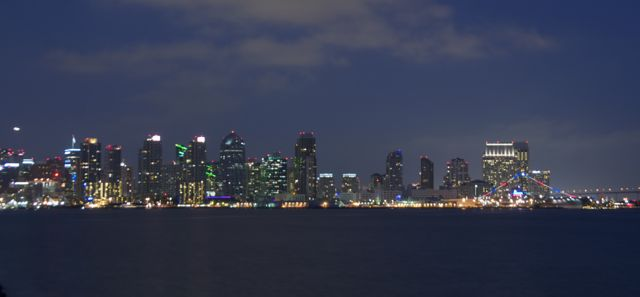
\includegraphics[width=0.5\textwidth]{sandiego}
%  \caption[Short figure caption (must be \protect{$< 4$} lines in the list of figures)]{A picture of San Diego.  Note that figures must be on their own line (no neighboring text) and captions must be single-spaced and appear \protect\textit{below} the figure.  Captions can be as long as you want, but if they are longer than 4 lines in the list of figures, you must provide a short figure caption.\index{SanDiego}} 
%  \label{fig:sandiego}
%\end{figure}

%\subsection{A Table Example}

%While in Section \ref{ssec:figure_example} Figure \ref{fig:sandiego} we had a majestic figure, here we provide a crazy table example.
%

%%%% TABLE 1 %%%%
%\vspace{0.25in}
%\begin{table}[!ht]
%\caption[Short figure caption (must be \protect{$< 4$} lines in the list of tables)]{A table of when I get hungry.  Note that tables must be on their own line (no neighboring text) and captions must be single-spaced and appear \protect\textit{above} the table.  Captions can be as long as you want, but if they are longer than 4 lines in the list of figures, you must provide a short figure caption.}

%\vspace{-0.25in}
%\begin{center}
%\begin{tabular}{|p{1in}|p{2in}|p{3in}|}
%
%\hline
%Time of day & Hunger Level & Preferred Food \\
%
%\hline
%8am & high & IHOP (French Toast) \\
%
%\hline
%noon & medium & Croutons (Tomato Basil Soup \& Granny Smith Chicken Salad) \\
%
%\hline
%5pm & high & Bombay Coast (Saag Paneer) or Hi Thai (Pad See Ew) \\
%
%\hline
%8pm & medium & Yogurt World (froyo!) \\
%
%\hline
%\end{tabular}
%\end{center}
%\label{tab:analysis3}
%\end{table}
%
%
%
%% APPENDIX
%\appendix
%\chapter{Final notes}
%What to do about things \cite{Martin_1983}.  What did he say \cite{Rilling_Insel_1999}.
%  Remove me in case of abdominal pain.



%% END MATTER
% \printindex %% Uncomment to display the index
% \nocite{}  %% Put any references that you want to include in the bib 
%               but haven't cited in the braces.
\bibliographystyle{alpha}  %% This is just my personal favorite style. 
%                              There are many others.
%\setlength{\bibleftmargin}{0.25in}  % indent each item
%\setlength{\bibindent}{-\bibleftmargin}  % unindent the first line
%\def\baselinestretch{1.0}  % force single spacing
%\setlength{\bibitemsep}{0.16in}  % add extra space between items
\bibliography{refs}  %% This looks for the bibliography in template.bib 
%                          which should be formatted as a bibtex file.
%                          and needs to be separately compiled into a bbl file.
\end{document}

